\documentclass[]{htwg-report}

\usepackage{geometry}
\usepackage{setspace}
\usepackage{hyperref}
\usepackage{listings}
\usepackage{xcolor}
\usepackage{graphicx}
\usepackage{booktabs}
\usepackage{caption}
\usepackage{float}
\usepackage{placeins}
\usepackage{dirtree}

\lstdefinelanguage{yaml}{
  keywords={true,false,null,y,n},
  keywordstyle=\color{blue}\bfseries,
  basicstyle=\ttfamily\small,
  sensitive=false,
  comment=[l]{\#},
  commentstyle=\color{gray}\ttfamily,
  morestring=[b]",
  morestring=[b]',
  stringstyle=\color{red},
  breaklines=true,
  frame=single
}

\lstset{
  basicstyle=\ttfamily\footnotesize,
  breaklines=true,
  breakatwhitespace=true,
  columns=fullflexible,
  keepspaces=true,
  showstringspaces=false,
  frame=single,
  rulecolor=\color{gray!30},
  xleftmargin=6pt,
  xrightmargin=6pt
}

\addbibresource{bib/books.bib}
\addbibresource{bib/websites.bib}

\begin{document}

%% Use Roman numerals for the page numbers of the title pages and table of
%% contents.
\frontmatter

%% 'reporttype' add background elements to the cover / front page
%% possible values are:
%% bachelor	--> B S C
%% master	--> M S C
%% other		--> none
\reporttype{bachelor}

\reporttypetext{Bachelor Thesis}

\title[Kubernetes-Evaluation]{Von Docker Compose zu Kubernetes: Evaluation der Zuverlässigkeit}
\author{Konstantin Leon Göke}
\studentnumber{307393}
\studentemail{konstantin.goeke@htwg-konstanz.de}

\doclocation{Deutschland}
\docdate{30. Juni 2026}

\makecover[]
%          
%% Include an optional title page.
\begin{titlepage}
\newgeometry{hscale=0.81,vscale=0.8}

\AddToShipoutPicture*{\BackgroundImgTitelPage}

\vspace*{12\bigskipamount}


%% Print the title in htwg-teal.
{\makeatletter
\fboxsep=0pt
\colorbox{htwg-white}{\begin{minipage}[t]{145mm}
    \begin{flushleft}
        %% Print Report Type Text
        \color{htwg-teal}\Huge{\@report@typetext}
        \\
        %% Print Report Title
        \color{htwg-teal}\Huge\textbf{\@title}
    \end{flushleft}
\end{minipage}}
\makeatother}

\bigskip
\bigskip

by
%door

\bigskip
\bigskip

%% Print the name of the author.
{\makeatletter
\Large\bfseries\@author
\makeatother}

\vfill

zum Erlangung des akademischen Grades

\bigskip
\bigskip

{\bfseries Bachelor of Science}

in Angewandte Informatik

\bigskip
\bigskip

an der Hochschule Konstanz Technik, Wirtschaft und Gestaltung

\vfill

\begingroup
\renewcommand*{\arraystretch}{1}
\rowcolors{2}{white}{white}
{\makeatletter
\begin{tabular}{lll}
    Martikelnummer: & \@student@number \\ \\
    Abgabedatum: & \@doc@date \\ \\
    Erstbetreuer: & \textbf{Prof.\ Dr.\ Marko Boger} \\
    Zweitbetreuer: & \textbf{Prof. \ Dr.\ Pascal Laube}
\end{tabular}
\makeatother}
\endgroup

\bigskip
\bigskip
Eine elektronische Version dieser Bachelorarbeit ist verfügbar unter \url{https://github.com/Spankyhsk/htwg-latex}.

%% reset page margins
\newgeometry{hscale=0.7,vscale=0.8}
\end{titlepage}



\input{abstract}

\tableofcontents

%% Use Arabic numerals for the page numbers of the chapters.
\mainmatter

\chapter{Einleitung}

Wir leben in einer Zeit der Digitalisierung. Immer mehr Bereiche des Lebens werden durch digitale Lösungen vorangetrieben.
Dazu gehören auch Lernveranstaltungen. Mithilfe von Webseiten wie Moodle können Vorlesungsinhalte sowie Testate digital angeboten werden.
Besonders in Fachbereichen wie der Informatik bietet es sich an, Vorlesungen und Klausuren zu digitalisieren, da der Code schließlich digital und nicht auf Papier ausgeführt werden soll.
Daher soll für den Kurs „Programmiertechnik 1” zukünftig die Lernplattform Codetask verwendet werden. 
Mit Codetask sollen Vorlesungen und Klausuren durchgeführt werden. Der Schwerpunkt von Codetask liegt auf der Programmiersprache Scala.
In den Vorlesungen werden Inhalte vorgetragen und passende Aufgaben zum Thema gestellt, die von den Studierenden bearbeitet werden sollen.
Zu diesen Aufgaben gehören Single-Choice-Fragen, Multi-Choice-Fragen, Textaufgaben und Lückentextaufgaben, die als „Koans” bezeichnet werden.
Eine weitere Aufgabenart, die bei Codetask eine Besonderheit ist, sind Codeaufgaben, bei denen die Studierenden einen funktionierenden Code schreiben müssen.
Dieser Code wird dann durch einen internen Compiler ausgewertet, um zu prüfen, ob er funktioniert. Diese Art der Aufgabe wird „Codetask” genannt.
Die gleichen Aufgabenarten sollen auch in den Klausuren gestellt werden.

Da Vorlesungen und insbesondere Klausuren mit Codetask durchgeführt werden sollen, muss Codetask auf einem zuverlässigen System betrieben werden.
Eine Klausur ist ein kritischer Bereich, in dem die Anwendung verfügbar bleiben muss.
Die Anwendung muss dabei stabil gehalten werden, damit es bei einer Klausur zu keinen Ausfällen kommt. Falls doch welche auftreten, muss die Anwendung schnell wiederhergestellt werden.
Fehler im System dürfen die Klausuren nicht beeinflussen.

Aktuell wird Codetask auf einem Docker Compose betrieben.
Ein Docker Compose bietet jedoch keine optimale Ausfallsicherheit, da jeder Service nur einmal ausgeführt wird und die gesamte Anwendung nur auf einem Server läuft.
Dadurch ist die Last der Anwendung auf einen Server ausgelegt und an dessen Grenzen limitiert.
Dabei ist inzwischen schon normalität, Anwendungen in verteilten Systemen zu betreiben. 
Der benötigte Ressourcenverbrauch erhöht sich schneller in der Gesellschaft, als die Hardwareentwicklung sich an diesen Ressourcenverbrauch anpassen kann.
Es ist aber oft auch günstiger, mehrere Hardware-Systeme mit normalem Ressourcenverbrauch zu beschaffen, als ein System, das einen größeren Ressourcenverbrauch verwalten kann.
Seine Anwendung auf mehrere Systeme zu verteilen, bringt aber nicht nur die Lastverteilung, sondern macht auch die Anwendung ausfallsicherer.
Fällt eine Hardware eines Systems aus, kann die Anwendung auf die andere Hardware weiterbetrieben werden.
Dadurch stellt sich die Frage, ob Codetask für die Produktionsumgebung in einem verteilten System besser aufgehoben ist.
Um Codetask in einem verteilten System zu betreiben, soll Kubernetes verwendet werden. Kubernetes selbst bietet dabei auch viele Features, mit denen die Zuverlässigkeit von Codetask zunehmen kann.

Daher beschäftigt sich diese Arbeit mit der Umstellung von Codetask von einer Docker-Compose-Umgebung auf eine funktionierende Kubernetes-Umgebung.
Zu diesem Zweck muss zunächst ein Kubernetes-Cluster im Hochschulnetzwerk ohne Cloud-Einbindung erstellt werden. Dieser soll so eingerichtet werden, dass eine höhere Zuverlässigkeit erzielt wird.
Abschließend sollen die Docker-Compose-Umgebung und die Kubernetes-Umgebung durch Tests verglichen werden. Dabei wird evaluiert, wie sich die Zuverlässigkeit in den Kategorien Verfügbarkeit, Fehlertoleranz, Stabilität und Wiederherstellbarkeit unterscheidet.

Zunächst werden die wichtigsten Grundlagen von Docker Compose und Kubernetes sowie die Faktoren, die die Zuverlässigkeit beeinflussen, vorgestellt. Anschließend wird erläutert, wie Kubernetes die Zuverlässigkeit verbessern kann.
Anschließend wird das aktuelle System, das mit Docker Compose betrieben wird, analysiert und vorgestellt.
Daraufhin wird die Implementierung der Kubernetes-Umgebung vorgestellt und dabei auch erörtert, wie sich dadurch die Zuverlässigkeit erhöhen kann.
Nach der Implementierung der Kubernetes-Umgebung werden beide Umgebungen mit Load- und Chaostests getestet und die Ergebnisse verglichen.
Zum Schluss folgt das Fazit, in dem die Einschätzung präsentiert wird, ob sich die Umstellung rentiert, und aufgezeigt wird, wie darauf aufgebaut werden kann.

\chapter{Grundlagen}

In diesem Kapitel werden die Grundlagen von Docker, Container-Orchestrierung und der Technologie, die hinter Kubernetes steckt, sowie der Begriff der Zuverlässigkeit behandelt.
Ziel ist es, ein besseres Verständnis für die Technologie zu vermitteln.

\section{Zuverlässigkeit}

Zuverlässigkeit bezeichnet die Wahrscheinlichkeit, mit der ein System über einen bestimmten Zeitraum hinweg erreichbar ist.
Dabei besteht Zuverlässigkeit aber nicht nur aus der Verfügbarkeit eines Systems, sondern auch aus dessen Fehlertoleranz, Stabilität und Wiederherstellbarkeit.

Die Fehlertoleranz beschreibt dabei nicht, dass keine Fehler passieren, sondern wie ein System mit Fehlern umgeht. Ein zuverlässiges System soll trotz Fehler weiterlaufen, ohne dass es zu Ausfällen kommt oder sich Fehler anderweitig bemerkbar machen.
Daher ist es bei der Zuverlässigkeit nicht am wichtigsten, dass ein System keine Fehler produziert, sondern dass es kontrolliert mit Fehlern umgehen kann.

Wenn es zu Ausfällen im System kommt – durch Fehler oder auch Updates –, muss das System automatisch darauf reagieren können, damit die Downtime möglichst gering ist.
Daher muss das System nach einem Ausfall wieder in seinen ursprünglichen, funktionierenden Zustand versetzt werden.

Zur Fehlervermeidung ist es wichtig, dass ein System stabil läuft, damit es funktionsfähig bleibt. 
Dazu gehört, dass ein System mit Last umgehen kann und sich entsprechend der Last hochskalieren kann, um eine Überlastung des Systems zu vermeiden.

Wenn ein System eine schlechte Performance hat, kann die Zuverlässigkeit geringer sein. Dies hängt damit zusammen, dass die Stabilität des Systems gefährdet wird, da mehr Last entsteht.

\section{Containerisierung}

Um über Docker und Kubernetes sprechen zu können, müssen zunächst deren grundlegende Technik, die Container, besprochen werden. 
Es muss geklärt werden, was sie erfüllen, wie sie funktionieren und wie sie sich von virtuellen Maschinen (zur Vereinfachung ab sofort VM genannt) unterscheiden.

Container sollen die Aufgabe erfüllen, dass eine Anwendung auf jeglichen Geräten laufen kann, unabhängig von Betriebssystem, Umgebungsvariablen, Einstellungen und Ähnlichem. 
Dadurch soll erreicht werden, dass eine Anwendung nicht nur auf dem eigenen Gerät, sondern auf jedem Gerät funktioniert.

Dazu werden die Anwendungen in einem Container gestartet. Dieser führt die Anwendung in einer isolierten Umgebung aus. 

Dieses Konzept wurde, aber nicht von Containern eingeführt, sondern gab es schon mit VMs davor. 
Es unterscheidet sich aber wie VMs und Container das umsetzen, da eine VM die gesamt benötigte Hardware mit Softwarekomponenten simuliert,
während Container direkt die Infrastuktur des Host-System mit nutzt, wie den Kernel. \parencite[vgl. 54]{kofler2023docker}

Dadurch sind Container ressourcensparender als VMs. Zudem lassen sie sich schneller aufbauen.
\section{Docker}
Docker ist aus der Welt der Container nicht wegzudenken. 
Zwar hat diese Firma die Container nicht erfunden, aber sie so weit verbreitet, dass sie als Synonym dafür benutzt werden, wie Lego für Klemmbrettbausteine

Ein Container wird durch ein Image erstellt. Die Besonderheit dabei ist, dass das Image ein Read-only-Dateisystem ist und daher im laufenden Container nie verändert werden kann.
Um ein Image zu erstellen, muss in Docker zunächst ein Dockerfile angelegt werden.

Eine weitere Besonderheit bei Containern sind die sogenannten Volumes. Bei Containern werden Dateien direkt im Host-System gespeichert. Diese Verzeichnisse sind vom Container getrennt.
Dadurch bleiben die Daten auch erhalten, wenn der Container neu eingerichtet wird.
Docker legt dabei normalerweise automatisch ein Verzeichnis an, wenn ein Container ein Volume benötigt.

Images müssen aber nicht immer, selber erstellt werden, sondern können auch extern aus dem Internet gezogen werden.
Dabei bietet sich bei Docker besonderes der Docker Hub an. In dieser von Docker betriebenen Platform können viele Image gefunden werden die von der Docker-Community erstellt wurden.
Dies kann wie ein Art Werkzeugkoffer angesehen werden, von dem vorgefertige Anwendungen und Umgebungen genutzt werden können oder sogar mit dem eigenen Image kombinierbar sind,
wie z.B. mongodb, nginx und so weiter \parencite[vgl. 50]{kofler2023docker}. 

Natürlich gibt es da auch wieder mehrere alternativen für den Docker Hub.
\section{Docker Compose}
Um eine Anwendung in einer isolierten Umgebung auszuführen, wird ein Container genutzt.
Wenn die eigene Anwendung aus mehreren Services besteht, wie es bei einer Microservice-Architektur der Fall ist, ist es weniger plausibel, alle Services in einen Container einzubauen. Stattdessen ist es sinnvoller, jeden Service in einen eigenen Container auszuführen.

Dadurch soll das Konzept der Separation of Concerns erreicht werden. 
Das Ziel besteht darin, einzelne Bestandteile einer Anwendung zu trennen, sodass sie isoliert und unabhängig voneinander funktionieren, z. B. Frontend, Backend und Datenbanken. Das bringt mehrere Vorteile.

Zum einen können sich Entwickler in mehrere Teams aufteilen. Ein Team konzentriert sich dann beispielsweise auf das Frontend, während ein anderes nur für das Backend zuständig ist. 
So muss sich nicht jeder mit allen Teilen auskennen.

Ein weiterer Vorteil dieser Isolation ist, dass der Code übersichtlicher ist, sich einfacher debuggen lässt und einfacher zu aktualisieren ist.
Dadurch beeinflussen Fehler nicht die gesamte Anwendung, sondern nur die eigenen Bereiche. Das ist auch bei Containern von Vorteil, da ein Fehler im Code oder in den Einstellungen des Containers nicht die gesamte Anwendung herunterfährt, sondern nur den Container dieses Services beeinflusst.

Zudem bringt die Isolation den Vorteil, dass Services wiederverwendet werden können. So kann beispielsweise ein Container für eine Datenbank für mehrere Anwendungen genutzt werden.

Um die Verwaltung der einzelnen Container zu vereinfachen, bietet Docker das sogenannte Docker Compose an.
Docker Compose (zur Einfachheit ab sofort Compose genannt) startet alle Container eines Services gleichzeitig, verwaltet diese und richtet ein Netzwerk zwischen ihnen ein.

Das Compose wird mit einer Compose.yaml-Datei eingerichtet.
Der allgemeine Aufbau einer solchen Datei ist ganz simpel: Zunächst werden unter dem Bezeichner „services” die verschiedenen Services aufgelistet. 
Darunter werden wiederum eigene Einstellungen für den Container definiert, beispielsweise Volumespfade, Netzwerkports oder Environment-Variablen.

\begin{lstlisting}[language=yaml, caption={Beispiel einer compose.yaml Datei}]
services:
    serviceName1:
        key1: einstellung
        key2: einstellung
        ...
    serviceName2:
        key1: einstellung
        key2: einstellung
        ... 
    ...
\end{lstlisting}

Compose kann Images direkt aus dem Internet mit dem Schlüssel „image“ ziehen, aber Compose kann auch Images mit dem Schlüssel „build“ bauen.
Dafür muss der Pfad des Dockerfiles angegeben werden und der Kontext, den der Build-Prozess erhalten soll.

Zusätzlich zu den Services können weitere Definitionen für Netzwerke und Volumes eingerichtet werden, die für die Container verwendet werden können.

Der Vorteil von Compose ist, dass es einfach zu nutzen ist und sehr einsteigerfreundlich ist.
Das liegt einerseits daran, dass Compose eine einfache .yaml-Datei ist, andererseits daran, dass Compose alle Container auf einem Host startet. Dadurch verwaltet Compose die Container direkt, alle Container befinden sich im gleichen Netzwerk und die Volumes befinden sich auf dem gleichen Gerät wie der Container. 
Dabei stößt Compose jedoch auch an seine Grenzen.

Ein Compose ist auf ein Gerät begrenzt. Das reicht zwar bei vielen Anwendungen aus, bietet aber kein Failover, wenn das Gerät ausfällt.
Zudem wird die gesamte Last nur auf diesem Gerät verteilt. 

Zusätzlich gibt es im Compose von jedem Container nur einen Replica. Daher kann es beim Ausfall oder Update eines Containers zu einer Downtime kommen.

\section{Container-Orchestrierung}
Compose kann als Single-Host-Container-Orchestrierung betrachtet werden, da es mehrere Container auf einem einzigen Host verwaltet und koordiniert.
Ein Single Host hat den Nachteil, dass es kein Failover gibt, wenn der Host ausfällt, und dass die gesamte Last, die durch die Services verursacht wird, nicht verteilt wird.
Um das zu verhindern, können die Services auf eine Gruppierung von Host-Rechnern, auch Cluster genannt, verteilt werden. Dies ist mit Compose jedoch nicht möglich.
Dafür wird eine Cluster-/Multi-Node-Container-Orchestrierung benötigt. Diese verwaltet die Container über Services, die eine weitere Abstraktionsebene über den Container darstellen.

\subsection{Docker Swarm}
Docker selber bietet als Cluster-Orchestrator Docker Swarm an (zureinfachheit absofort nur Swarm genannt) und ist so mit einer der einfachsten Wege um
vom einen Compose zu einen Cluster-Orchestrator zuwechseln, da weiterhin die compose.yaml verwendet wird.

Die compose.yaml Datei muss dafür mit dem Befehl docker stack deploy ausgeführt werden, dabei setzt Swarm aber vorraus, dass das Gerät zu einen Cluster gehöhrt bzw 
wie es in Swarm heißt, einen Docker-Swarm. Es würd aber nicht verlangt, das der Swarm schon aus mehreren Host besteht,
sondern kann mit dem Befehl docker swarm init, ein Swarm mit nur einen Host auf den Rechner erstellt werden \parencite[vgl. 119]{kofler2023docker}, 
daher kann Swarm auch nur auf einen Node verwendet werden, auch wenn es als Multi-Node ausgelegt ist.

Dennoch besteht ein Swarm immer aus zwei verschiedenen Arten von Nodes. 
Einerseits gibt es die Manager Nodes, die die Cluster-Verwaltung übernehmen, andererseits gibt es die Worker Nodes, auf denen die Container ausgeführt werden. 
Ein Manager Node kann aber auch zusätzlich als Worker Node verwendet werden, beispielsweise wenn der Swarm nur aus einem Node besteht.

Die Vorteile von Swarm im Vergleich zu Compose sind zum einen, dass Swarm direkt auf mehrere Nodes skaliert werden kann und dass die Replikate der Container nun hochskaliert werden können. 
Swarm sorgt mit seiner Cluster-Verwaltung außerdem dafür, dass die Anzahl der Replicas der Container immer gleich bleibt, auch wenn ein Container oder sogar ein ganzer Node ausfällt.
Dieser Zustand wird als Desired-State-Prinzip bezeichnet.

Obwohl Swarm einen einfachen Übergang zu einer Cluster-Orchestrierung bietet, ist es dennoch nicht die optimale Wahl als Cluster-Orchestrator.
Einerseits ist die Anwendung weiterhin an Docker-Techniken gebunden, andererseits ist Swarm nicht so stark verbreitet, weswegen es eine kleinere Community hat.
Dadurch ist Swarm weniger erweiterbar und flexibler als andere Cluster-Orchestratoren.

\subsection{Kubernetes}

Kubernetes bietet mit einer größeren Community, vielen guten Erweiterungen und ausführlichen Domkumentationen
zum vergleich zu Swarm, trotz höhrer Komplexität, gute Vorteile \parencite[vgl. 452]{kofler2023docker}.
Dabei darf Kubernetes nicht als Erweiterung von Docker angesehen werden, sondern als eigenständiges System.
Kubernetes verwendet eine Container Runtime Interface (CRI), weshalb weitere Runtimes verwendet werden können. Dadurch ist Kubernetes nicht auf Docker beschränkt.

Daher wird sich dieser Teil zuerst mit der Architektur beschäftigen und anschließend die Objekte und Ressourcen von Kubernetes vorstellen.

\input{chapters/grundlagen/cluster-orchestrator/kubernetes/architektur.tex}
\input{chapters/grundlagen/cluster-orchestrator/kubernetes/manifeste.tex}
\input{chapters/grundlagen/cluster-orchestrator/kubernetes/pods.tex}
\input{chapters/grundlagen/cluster-orchestrator/kubernetes/deployments.tex}
\input{chapters/grundlagen/cluster-orchestrator/kubernetes/services.tex}
\input{chapters/grundlagen/cluster-orchestrator/kubernetes/ingress.tex}
\subsection{Zuverlässigkeit durch Kubernetes}

Kubernetes bietet durch seine Technik einige Features, die genutzt werden können, um die Zuverlässigkeit zu erhöhen.

Dies beginnt damit, dass Kubernetes mehrere Replikate von Pods hat, wodurch sich die Verfügbarkeit verbessert. Selbst wenn ein Pod eines Services ausfällt, z. B. eines Backends, ist dieser dennoch verfügbar, da der Traffic auf die Replikate umgeleitet wird.
Dies kann durch die Eigenschaft von Kubernetes als Cluster-Container-Orchestrator gesteigert werden, da die Anwendungen auf mehreren Nodes laufen. Deshalb bleibt die Anwendung auch bei einem Node-Ausfall bestehen, während bei einem Single-Host-Container-Orchestrator die gesamte Anwendung down wäre.
Dies kann bei Kubernetes auch verknüpft werden, indem im Deployment eingestellt wird, dass sich die Replicas von Pods desselben Services auf verschiedene Nodes verteilen. Dadurch bleibt der Service auch bei einem Node-Ausfall erreichbar.
Dabei punktet Kubernetes auch beim Aspekt der Fehlertoleranz, da es erkennt, wenn ein Pod ausfällt – egal aus welchem Grund – und den Traffic auf die noch existierenden Replicas dieses Pods umleitet.

Kubernetes verfolgt das Desired-State-Prinzip, weshalb es bei einem Pod-Ausfall direkt versucht, den Pod wiederherzustellen, damit die Anzahl der Replicas dieses Pods gleich bleibt, wie es im Deployment angegeben ist.
Bei einem Ausfall eines ganzen Nodes versucht Kubernetes, die Pods auf einem anderen Node wiederherzustellen. Sobald ein neuer Node im System hinzugefügt wird oder der alte Node wiederhergestellt wurde, kann Kubernetes diese Pods erneut verteilen.

All dies gehört auch zum Self-Healing von Kubernetes und kann die Zuverlässigkeit von Anwendungen weiter verbessern.
Kubernetes überwacht die Gesundheit der Pods durch Probes. Dadurch kann erkannt werden, ob der Container im Pod noch richtig läuft. Falls nicht, würde Kubernetes den Pod als ungesund markieren und den Traffic auf die anderen Pods dieses Services umleiten.
Zusätzlich versucht Kubernetes, den Container im Pod oder sogar den ganzen Pod neu zu starten.  Dadurch können Fehler im System vermieden und der richtige Betrieb wiederhergestellt werden.

Das Desired-State-Prinzip muss in Kubernetes aber nicht fest sein, sondern kann auch automatisch nach Last skaliert werden, und zwar durch den Horizontal Pod Autoscaler. 
Dieser kann die Anzahl der Replicas eines Pods erhöhen und auf eine angegebene maximale und minimale Anzahl beschränken, je nachdem, wie viel Last ein Service verbraucht.
Dies verstärkt die Stabilität im System, da die Ressourcen angemessen verteilt werden.

Kubernetes erhöht auch die Zuverlässigkeit durch Rolling Updates. Bei einem Rolling Update wird ein Pod nach dem anderen ausgetauscht, während das Update läuft. Dadurch können Ausfälle während einer Aktualisierung vermieden werden.
Dies kann durch die Probes, die im Self-Healing verwendet werden, verbessert werden, indem zuerst geprüft wird, ob der Pod gesund ist, bevor er für den Traffic freigegeben wird.

\chapter{Systemanalyse}

In diesem Kapitel wird die bestehende Struktur und das Deployment von Codetask zum Start der Arbeit kurz analysiert und vorgestellt.

Dabei wird zuerst die Architektur und die Services von Codetask kurz vorgestellt, um anschließend zu zeigen, wie es deployt wird. Dazu gehört das Docker-Compose sowie die VM, auf der Codetask läuft.

\section{Architektur Codetask}

Codetask besteht aus einer Microservice-Architektur, die grundlegend aus sieben Services besteht.

Das Backend besteht dabei aus drei Services. Dazu gehört die Haupt-API, aber auch die Check-API, in der ein Scala-Compiler läuft, um Code live auszuführen. In der sogenannten Codetask-Aufgaben können Anwender Code schreiben und prüfen, ob dieser korrekt ist.
Da Code live ausgeführt wird, wurde dieses Feature in der Check-API isoliert, damit die Haupt-API nicht angegriffen werden kann.
Die Haupt-API und die Check-API verwenden das Play3-Framework und auch Scala 3.
Der dritte Service für das Backend ist die AI-API. Diese wird genutzt, damit Studierende beim Bearbeiten von Aufgaben eine KI um Hilfe bitten können.
Aufgrund der für diese Implementierung benötigten Abhängigkeiten ist die AI-API in Scala 2 geschrieben und nutzt das Play2-Framework. Aus diesem Grund wurde sie von der Haupt-API isoliert.
Die Haupt-API und die AI-API sind auch von außen erreichbar und haben ihre eigene Host-DNS.
Alle drei APIs nutzen sbt als Build-Tool und da alle drei mit Scala geschrieben sind, sind diese auch stateless, da Scala eine funktionale Programmiersprache ist.

Für das Frontend werden zwei Services verwendet. Ein Service ist das Webframework, das aus dem Vue3-Framework besteht, der andere Service ist der dazugehörende Webserver nginx.

Die Datenbank ist ebenfalls ein eigener Service. Als Datenbanksystem wird die NoSQL-Technik MongoDB in der Version 6.0.0 verwendet, die das EOL erreicht hat.
Um die Verwendung von MongoDB zu vereinfachen, gibt es als Service auch Mongo-Express. Mit diesem kann die MongoDB-Anwendung über eine WebUI verwendet werden.

In der Produktions- und Staging-Umgebung gibt es zusätzlich den Service Traefik, der als Reverse Proxy verwendet wird.

Die Aufgaben von Codetask werden in eigenen GitLab-Repositories angelegt und gespeichert. Der Inhalt wird von der Haupt-API abgerufen und dann in der Datenbank gespeichert.
Dabei gibt es zwei verschiedene GitLab-Repos. Einmal ein öffentliches, in dem der Inhalt der Vorlesungen vorhanden ist, und ein privates, in dem Klausuren erstellt und gespeichert werden. 
Das private GitLab-Repository ist jedoch noch nicht im Code eingebunden. Damit die Haupt-API auf die Repos zugreifen kann, wird ein Token verwendet.

Alle GitLab-Repos liegen nicht auf der HTWG-Instance, sondern in der öffentlichen GitLab-Instance.
\section{Deployment Codetask}

Codetask verfügt über drei verschiedene Umgebungen: eine Local-, eine Staging- und eine Prod-Umgebung. 
Jede dieser Umgebungen hat ihre eigene Compose-Datei. Für die Haupt-API, die Check-API, die AI-API und das Webframework sind eigene Dockerfiles angelegt, wobei jeweils für die lokale Umgebung ein eigenes Dockerfile verwendet wird. 
Jede dieser Umgebungen hat eine eigene .env-Datei, in der Passwörter, Tokens und weitere Variablen stehen, die im Code aufgerufen werden.

Im Ordner .deployment gibt es die Datei mongo-init.js, die verwendet wird, um die MongoDB zu initialisieren.
\begin{figure}[htbp]

\dirtree{%
.1 teamprojekt/.
.2 .deployment/.
.3 prod/.
.4 docker-compose.yml.
.3 staging/.
.4 docker-compose.yml.
.3 mongo-init.js.
.2 .docker/.
.2 ai-api/.
.2 api/.
.2 check-api/.
.2 web/.
.3 frontend/.
.2 docker-compose.yml.
}

\caption{Vereinfachtes Projektverzeichnis der Codetask-Anwendung}
\label{fig:projektstruktur}

\end{figure}

\FloatBarrier
\subsection{Lokale Umgebung}

Die Docker-Compose.yml-Datei für die lokale Umgebung liegt im Root-Verzeichnis des Projekts.
Sie dient dazu, dass Codetask lokal ausgeführt werden kann, um daran zu entwickeln und Veränderungen auszuprobieren, bevor diese gepusht werden.
Daher sind alle Services unter localhost erreichbar, bekommen aber vom Compose jeweils eigene Ports zugeordnet. Es werden keine weiteren Netzwerkeinstellungen eingerichtet.

Das Compose der lokalen Umgebung baut die Images mit den selbst erstellten Dockerfiles selbst und nimmt dabei das Root-Verzeichnis als Kontext.
Die Anwendungen in den Containern werden jeweils im DEV-Modus gestartet, wodurch das Webframework beispielsweise einen eigenen Webserver hat. Dadurch verbrauchen alle Container jedoch mehr Ressourcen als im Normalbetrieb.
Die Images von nginx, mongodb und mongo-express werden aus dem Internet gezogen. 

Alle Services haben die Option „restart: unless-stopped” hinzugefügt bekommen, wodurch Container, wenn sie ausfallen, direkt neu gestartet werden.

Die Services haben ein Env-File zugeordnet bekommen, aber manche haben direkt eigene Environment-Variablen im Compose. Das Besondere an der lokalen Umgebung ist, dass die Volumes der Konfiguration der Services im Container überschrieben werden, wodurch die Konfiguration außerhalb des Containers angepasst werden kann, während dieser läuft, und nach einem Neustart verwendet werden kann.
\subsection{Staging und Production Umgebung}

Die Docker-Compose-Dateien sind im Unterordner /.deployment zu finden.
In der Produktionsumgebung läuft die aktuelle Live-Version von Codetask, während die Staging-Umgebung einen Zwischenstand zwischen der lokalen und der Produktionsumgebung darstellt.
In dieser können Implementierungen und Entwicklungen in einer live-ähnlichen Umgebung getestet werden.

Die Compose-Dateien ähneln denen der lokalen Umgebung, haben dennoch deutliche Unterschiede.
So gibt es beispielsweise einen weiteren Service namens Traefik, der als Reverse Proxy benutzt wird. 
Die Umgebungen haben auch einen Eintrag des DNS-Servers der HTWG, wodurch sie auch von außen erreichbar sind. Die Staging-Umgebung ist hingegen nur über VPN erreichbar.
Der Host der Prod-Umgebung ist codetask.in.htwg-konstanz.de, der Host der Staging-Umgebung ist staging-codetask.in.htwg-konstanz.de. Wird der Host für die API oder AI-API verwendet, wird jeweils das Passende vorne dran gehängt, z. B. „api.codetask.in.htwg-konstanz.de”.
Daher haben beide Umgebungen jeweils drei URLs, wodurch drei Services von außen erreichbar sind. Die restlichen Services sind nur intern im Compose-Netzwerk erreichbar.
Bei der Produktionsumgebung haben alle drei URLs ein TLS-Zertifikat erhalten, wodurch jede mit HTTPS genutzt werden kann. Bei der Staging-Umgebung hat nur die URL für das Webframework ein TLS-Zertifikat erhalten.

Anders als bei der lokalen Umgebung werden die Images bei beiden Compose nicht mehr mit Dockerfiles selbst gebaut, sondern über die Container Registry vom GitLab-Repository von Codetask geholt.
Die Staging- und Produktionsumgebung haben auch ein anderes Dockerfile als die lokale Umgebung. Ein Unterschied ist beispielsweise, dass die Container nicht im DEV-Modus laufen oder dass im Frontend-Dockerfile ein Container für das Webframework und den Webserver enthalten ist.
\chapter{Implementierung}

In diesem Kapitel wird die Implementierung und Migration von Compose Deployment zu Kubernetes Deployment beschrieben.
Dabei beginnt es mit einer Migration von Codetask und der Einrichtung von zwei Clustern, um schließlich ein GitOps einzurichten.
Bei jedem Schritt werden das Ziel, die verwendeten Tools, die Umsetzung, die dabei aufgetretenen Probleme und die Ergebnisse präsentiert. 
Am Ende steht ein Kubernetes-Cluster, der als Produktionsumgebung genutzt werden kann.

\section{Migration der Compose-Anwendung}
Zunächst musste Codetask migriert werden, damit es in einen Kubernetes-Cluster deployt werden kann.
Das Ziel bestand also darin, das vorhandene Docker Compose in Helm Charts umzuwandeln.

\subsection{Verwendete Technologien/Werkzeuge}
\input{chapters/implementierung/migration/Kompose.tex}
\input{chapters/implementierung/migration/helm.tex}
\subsection{Umsetzung / Konfiguration}

Die erste Umsetzung besteht darin, aus einer der vorhandenen Docker-Compose-Dateien Manifeste zu erstellen.
Um den Prozess zu vereinfachen und zu beschleunigen, habe ich mich entschieden, das Tool Kompose zu verwenden.
Ich entschied mich dabei für die Compose.yml-Datei der lokalen Umgebung. 
Da diese im Root-Verzeichnis liegt, war es einfacher, sie mit Kompose zu verwenden. Zusätzlich benötigt das lokale Compose im Gegensatz zu den anderen beiden Composes keine externen Dateien, abgesehen von der mongo-init.js.
Ein weiterer Grund, warum ich mich für das lokale Compose entschieden habe, ist, dass es einen Service weniger hat als die anderen beiden Compose.

Nun musste ich im Root-Verzeichnis des Projekts nur den Befehl „Kompose convert“ eingeben und schon hatte ich zu jedem Service im Compose passende Manifeste, die auf die Compose-Datei basieren. Ausgenommen war mongo-express, da dieser zu diesem Zeitpunkt auskommentiert war. Dieser war aber nicht vonnöten.
Zu den Manifesten gehörten jeweils ein Deployment, ein Service und falls nötig ConfigMaps.

ConfigMaps sind Konfigurationen in Form von Key-Value-Pairs für die Container. Sie können für Env-Variablen oder, wie bei Codetask, zur Veränderung von Konfigurationen verwendet werden, ohne dass der Container neu deployed werden muss, wie es schon im Compose der Fall war.
Das hatte den praktischen Nutzen, dass ich die Konfiguration der Anwendungen an Kubernetes anpassen konnte, ohne den aktuellen Betrieb zu stören.
Empfindliche Daten wie z. B. Passwörter oder Token sollten aber nicht in ConfigMaps, sondern in Secrets gespeichert werden. Diese sind wie ConfigMaps, nur dass die Daten verschlüsselt im Cluster gespeichert sind.

Nach der Erstellung der Manifeste werden alle auf das Root-Verzeichnis des Projekts gelegt. Um mehr Ordnung zu schaffen, wurde im nächsten Schritt für jeden Service ein Helm Chart erstellt.
Die Helm-Charts wurden jedoch nicht in einem eigenen Repository gespeichert, sondern im Ordner „./charts” im Projektverzeichnis. Für jeden Service wurde ein Ordner erstellt, in dem eine Chart.yaml-Datei angelegt wurde, in der Organisationsinformationen wie Name und Version des Charts gespeichert werden. Zusätzlich wurde ein weiterer Unterordner namens „templates” erstellt, in dem die Manifeste des jeweiligen Services gespeichert wurden.
Somit verfügt das Projekt nun über Helm-Charts für API, AI-API, Check-API, Frontend, MongoDB und NGINX. Der Helm-Chart von nginx wurde jedoch direkt entsorgt, da dieser durch einen vorgefertigten Helm-Chart ersetzt werden soll.

Für MongoDB habe ich mich jedoch entschieden, das eigene Helm-Chart zu behalten, um bei der Datenbank mehr Kontrolle zu behalten, da der MongoDB-Driver des Projekts zu dem Zeitpunkt nicht neuere MongoDB-Versionen verwenden konnte.
Für das MongoDB-Chart musste dennoch eine Überarbeitung durchgeführt werden, da MongoDB als Datenbank keine stateless Anwendung ist und ein Deployment daher die falsche Wahl ist.
Daher wurde das Deployment, das Kompose für Mongodb erstellt hat, um einen StatefulSet ergänzt.

Ein StatefulSet unterscheidet sich von einem Deployment dadurch, dass es behutsamer mit den Pods umgeht. Pods haben in einem StatefulSet eindeutige Identifikationen, die auch nach einem Neustart bestehen bleiben und aus Pod-Name und Index bestehen.
Pods werden in einem StatefulSet auch in einer festen Reihenfolge erstellt und wieder gelöscht.
StatefulSets verwenden direkt Persistent Volumes und Persistent Volume Claims. Diese werden benötigt, um langfristig persistente Daten zu speichern und zu verwalten.

Nachdem das Deployment von MongoDB durch einen StatefulSet ersetzt wurde, wurde für jede Helm-Chart-values.yaml-Datei eine neue Version angelegt und die Manifeste so angepasst, dass die Key-Value-Zuordnung funktioniert. Dafür haben alle Keys in der values.yaml-Datei die gleichen Werte erhalten, die zuvor im Manifest standen.
Das Besondere an Helm ist dabei aber nicht nur, dass eine solche Ordnung eingebaut werden kann, sondern auch, dass beispielsweise If-Verzweigungen genutzt werden können. Es wurden If-Verzweigungen für Werte genutzt, die nur in einer lokalen Umgebung genutzt werden müssen, z. B. um die Konfigurationen für die Container zu überschreiben, damit diese verändert werden können, ohne dass die Container neu bereitgestellt werden müssen.

Es wurde gegen ein Umbrella Chart entschieden. Das ist ein Helm-Chart, das alle Helm-Charts, die benutzt werden sollen, als Abhängigkeit enthält, wodurch eine Anwendung ein zentrales Helm-Chart besitzt.
Diese Entscheidung wurde getroffen, damit die Services unabhängig voneinander bleiben.
\subsection{Probleme und Anpassungen}

Bei dieser Umsetzung gab es keine größeren Probleme, da durch die Hilfe von Kompose die Umwandlung von Compose zu Manifesten vereinfacht wurde. Zwar mussten Kleinigkeiten korrigiert und für MongoDB das Deployment mit einem StatefulSet angepasst werden, doch das war leicht zu bewältigen und durch die Warnungen der Kompose-Entwickler auch keine größere Überraschung.
\subsection{Ergebnisse der Umsetzung}

Nach Abschluss dieser Umsetzung kann Codetask nun in Kubernetes-Clustern bereitgestellt werden. Durch Helm wurde auch die Verwaltung und Wiederverwendbarkeit der Manifeste verbessert, wodurch deren Weiterentwicklung und Verwendung einfacher und übersichtlicher ist.

Da jeder Service ein eigenes Helm-Chart ist, kann nun jeder Service einzeln statt alle zusammen deployt werden.
\section{Aufbau der lokalen Kubernetes-Testumgebung}

Nachdem Codetask so angepasst wurde, dass es in einen Kubernetes-Cluster deployt werden kann, musste dies ausprobiert und weiterentwickelt werden, um Features von Kubernetes einbauen zu können.
Zu diesem Zweck sollte eine Kubernetes-Testumgebung erstellt werden, die einen Kubernetes-Cluster lokal auf dem Rechner simuliert.
Ziel dabei war, dass die Studierenden, die an diesem Projekt entwickeln, ihre Veränderungen testen können, ohne dass sie erst lernen müssen, wie ein Kubernetes-Cluster funktioniert bzw. verwendet werden muss.
Dabei war es mir auch wichtig, die Einrichtung so einfach wie möglich zu gestalten, damit auf den Rechnern der Studierenden so wenig wie möglich eingerichtet werden muss und diese schneller mit der Entwicklung beginnen können.
In der Vergangenheit hat das lokale Deployment von Codetask den Anfang sehr ausgebremst.
Ein weiteres Ziel ist es, die Manifeste zu erweitern, um diese in Kubernetes besser nutzbar zu machen.

\subsection{Verwendete Technologien/Werkzeuge}

\input{chapters/implementierung/localCluster/kind.tex}
\input{chapters/implementierung/localCluster/traefik.tex}
\subsection{Umsetzung / Konfiguration}

Kind kann einfach mit einem Install-Tool wie Chocolate heruntergeladen werden.
Um Kind mit mehreren Nodes laufen zu lassen, wurde eine Kind-Konfiguration erstellt, die beim Starten eines Kind-Clusters mitgegeben wird.
Der lokale Cluster hat einen Master-Node und zwei Worker-Nodes. 
Diese Aufteilung dient nur dazu, die Nutzung mehrerer Nodes zu simulieren und zu verhindern, dass die gesamte Last in einem Docker-Container liegt. 

Sobald der Cluster hochgefahren ist, müssen die Helm-Charts in den Cluster geladen werden. 
Danach werden die Images der eigenen Services in ein In-Cluster-Registry geladen. Anschließend wird ein Rollout der Deployments ausgeführt, damit die Pods die neuen Container wahrnehmen.

Damit die Studierenden den Cluster nicht selbst auf ihren lokalen Geräten einrichten müssen, wurde ein Automatisierungsskript entworfen. Für Windows ist dieses Skript in PowerShell geschrieben, während es für macOS und Linux in Shell geschrieben ist.
Das Automation-Script richtet den Kind-Cluster auf dem lokalen Gerät ein, lädt die Helm-Charts in den Cluster und erstellt daraufhin die Images, die in das In-Cluster-Registry gepusht werden. Zum Schluss führt es ein Rollout aus, damit die Deployments die Pods mit den Containern neu starten. 

Durch den lokalen Cluster konnten die eigenen Helm-Charts zunächst ausprobiert und angepasst werden.
Da im lokalen Cluster nur die Helm-Charts und der Code ausprobiert werden müssen und der Cluster nur eine kurze lebig ist, gibt es von jedem Service nur einen Pod.
Das hat auch weiterhin den Nutzen, dass auf den lokalen Geräten der Studierenden, die sich mit diesem Projekt befassen, weniger Ressourcen benötigt werden.

Die erste Anpassung, die der lokale Cluster an den Helm-Charts vorgenommen hat, war das Hinzufügen des Ressourcenmanagements.
In Kubernetes kann für die Pods angegeben werden, wie viel Ressourcen mindestens reserviert werden können und wie viel ein Pod maximal haben darf. 
Zu diesen Ressourcen gehören die benötigte RAM- und CPU-Kapazität. Dadurch kann Kubernetes die Pods besser verwalten, da nun bekannt ist, wie viel Ressourcen ein Pod mindestens braucht, es aber auch ein Limit gibt, damit kein Pod die Ressourcen anderer abziehen kann.
Um zu entscheiden, wie viel RAM und CPU jeder Pod bekommt, wurde ein Monitoring eingesetzt.

Die weitere Anpassung, die vorgenommen wurde, ist, dass Probes für jeden Helm-Chart hinzugefügt werden.
Dabei wurde für jeden Helm-Chart eine StartupProbe und eine ReadinessProbe eingerichtet. 
Eine StartupProbe prüft, ob der Container im Pod hochgefahren ist und die Anwendung gestartet wurde. Solange die StartupProbe nicht bestanden wurde, werden die anderen Probes blockiert.
Wenn eine StartupProbe zu oft fehlschlägt, wird der gesamte Pod neu gestartet.
Eine ReadinessProbe prüft, ob der Container Requests bearbeiten kann, d. h., ob die Anwendung selbst läuft und externe Services noch erreichbar sind, ohne die die komplette Anwendung nicht funktioniert.
Wird eine ReadinessProbe nicht bestanden, wird der Pod auf „NotReady” gesetzt. Dadurch wird der Traffic auf die anderen Pods umgeleitet, bis die ReadinessProbe wieder bestanden wird oder der Pod neu gestartet wird.

Dabei schickt Kubernetes die Probes als Request an die Pods selbst.
Beim Frontend muss nur dem Webserver ein einfacher Request geschickt werden, der mit einem 200-Statuscode beantwortet werden muss.
Bei der Haupt-API, der Check-API und der AI-API mussten eigene Healthcheck-Endpunkte implementiert werden. Diese antworten mit einem 200, wenn sie erreicht werden.
Die MongoDB wird über TCP-Sockets angefragt.

Damit die Service-Frontends, die Haupt-API und die AI-API von außen erreichbar sind, musste für jedes dieser Helm-Charts ein Ingress erstellt werden. 
Da geplant ist, Traefik als Ingress-Controller zu nutzen, wird dessen Helm-Chart auch schon in den lokalen Cluster geladen, um näher an der Produktionsumgebung zu bleiben.
Da die Nodes in Docker-Containern sind, musste über die kind config ein externPortMapping eingerichtet werden, damit die Ingress-Ports von außen über localhost erreichbar sind.
\subsection{Probleme und Anpassungen}
Beim Einrichten des lokalen Clusters sind Probleme aufgetreten.
Das erste Problem das entstanden ist war das lokale Registry der Images. Zwar hat kind eine eigene Lösung dafür, diese funktoniert aber unter Windows nur über den WSL, was gegen das Ziel sprach, dass der Lokale Cluster schnell und simple eingerichtet wird sprach, 
zum weitern arbeitet kind aktuell an einer bessern build-in Lösung für das lokale Registry \parencite{kind_local_registry}.
Daher wurde zunächst das Feature benutzt, bei dem die Images einfach in Kind geladen werden können. Dies war jedoch aufgrund der drei Nodes speicher- und RAM-intensiv, da die Images jeweils in alle drei Container geladen wurden.
Schlussendlich wurde sich daher für ein In-Cluster-Registry entschieden, wodurch das Container Registry in der lokalen Umgebung im Cluster ist.

Ein weiteres Problem entstand durch die Probes. Da die Healthchecks von den Pods selbst durchgeführt werden und die Pods im Kubernetes-Netzwerk eine eigene IP-Adresse haben, standen sie nicht in der Whiteliste der Play-Config, wodurch die Probes ständig fehlschlugen.
Da die Pods kurzlebig sind und bei einem Neustart ihre IP-Adresse verändern, konnte diese auch nicht in die Play-Config hinzugefügt werden. Daher musste in die White List der Play Config eine Wildcard eingefügt werden, um alle Pods zu erlauben. Da die Pods nur intern im Kubernetes-Netzwerk erreichbar sind und nur von außen über Ingress, entsteht dadurch aber kein Sicherheitsrisiko.

Bei der Einrichtung der Ingress gab es für den lokalen Cluster auch Probleme durch den Hostnamen. Da alle drei Services zunächst als Host „localhost” hatten, mussten diese mit Prefixen, die abgeschnitten wurden, unterschieden werden.
Die Präfixe wurden abgeschnitten, was zu Problemen bei den WebSockets der ai-API geführt hat. Dadurch wurden unterschiedliche Hosts benötigt.
Damit dennoch localhost als Basis verwendet werden kann und die Studierenden nichts in ihren Host-Dateien verändern müssen, startet die Automation zusätzlich einen DNS-Resolver mit einer DNS-Wildcard, damit verschiedene Hosts verwendet werden können.
Damit es plattformübergreifend ist, läuft dieser DNS-Resolver in Docker.
\subsection{Ergebnisse der Umsetzung}
Durch die Umsetzung haben die Studierenden einen lokalen Cluster, in dem sie ihre Implementierungen in einer produktionsechten Umgebung ausprobieren können.
Die Automation der Cluster-Einrichtung bringt nicht nur den Vorteil, dass die Studierenden den Cluster leicht auf ihren Geräten einrichten können, ohne Kubernetes-Kenntnisse zu benötigen, sondern der Cluster muss dadurch auch nur temporär auf diesen Geräten vorhanden sein, wenn er gerade benötigt wird. 
Dadurch können die Studierenden beim Entwickeln den Cluster mit nur einem Befehl starten, ihre Implementierungen testen und nach Abschluss der Arbeit diesen wieder mit einem Cleanup-Befehl entfernen, bis sie den lokalen Cluster wieder benötigen.

Durch die Ressourcenverwaltung können nun Pods besser auf den Nodes verteilt werden, zusätzlich wird auch verhindert das ein Service alle Ressourcen für sich selbst beanspruchen kann.
Zusammen mit den Probes und den RollingUpdates erzielt das Codetask bei einem Update eine Zero Downtime.

Durch den Ingress sind nun drei Services nach außen erreichbar mit http, während die anderen Services nur im Cluster selbst erreichbar bleiben.
\section{Aufbau des k3s-Clusters}
Der eingerichtete lokale Cluster dient zum Testen von Implementierungen in einer praxisnahen Umgebung und kann daher als DEV-Cluster bzw. -Umgebung angesehen werden.
Nun musste ein Cluster für die Produktionsumgebung eingerichtet werden.
Der Cluster soll nicht in einer Cloud, sondern im Hochschulnetzwerk betrieben werden. 
Dies ist zum einen eine finanzielle Entscheidung, zum anderen dient es der Absicherung der Privatsphäre, damit die Klausurnoten nur im Hochschulnetzwerk gespeichert sind.

Anders als beim Dev Cluster ist beim Prod Cluster eine hohe Zuverlässigkeit wichtig. 
Um diese zu erreichen, wird eine High-Availability-Architektur (im Folgenden HA-Architektur genannt) eingesetzt.
Eine HA-Architektur besteht dabei aus mindestens drei Master-Nodes und zwei Worker-Nodes.
Zusätzlich verfügt eine HA-Architektur über zwei Load Balancer (kurz LB genannt). 

Ein Load Balancer außerhalb des Clusters ist für die Kubernetes-Komponenten zuständig.
Da es nun mehrere Master-Nodes gibt, werden die Anfragen von den Worker-Nodes oder kubectl nicht mehr direkt an den Master-Node gestellt, sondern über den Load Balancer, der die Anfrage an die Master-Nodes verteilt.
Dadurch müssen die Clients nicht erst wissen, welche Master-Nodes aktuell erreichbar sind.

Der andere LB ist innerhalb des Clusters und verteilt den Anwendungs-Traffic auf die Pods.

\begin{figure}[htbp]
\centering
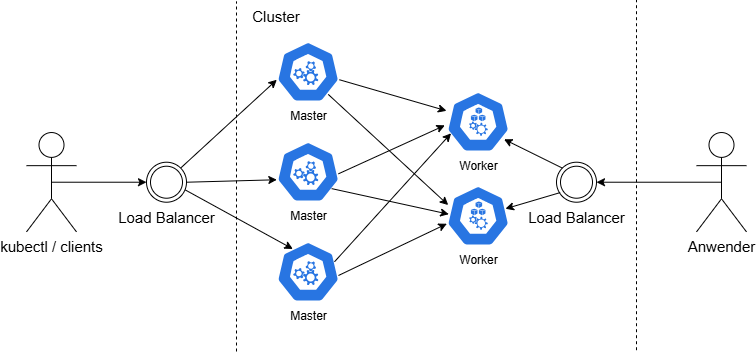
\includegraphics[width=0.8\textwidth]{bilder/implementierung/HAarchitektur.png}
\caption{High-Availability Architektur}
\label{fig:HAarchitektur}
\end{figure}

Das Ziel ist bei dieser Umsetzung einen Kubernetes Cluster mit einer HA Architektur im Hochschulnetzwerk einzurichten.
\FloatBarrier

\subsection{Verwendete Technologien/Werkzeuge}

\input{chapters/implementierung/prodCluster/k3s.tex}

\subsection{Umsetzung / Konfiguration}
Für die Einrichtung des Clusters im Hochschulnetzwerk hat die IT sechs VMs mit dem Betriebssystem Ubuntu bereitgestellt.
Auf einer der VMs wird der Load Balancer (LB) für die Verteilung der Anfragen zu den Master Nodes eingerichtet. Auf drei weiteren VMs werden die Master Nodes und auf den letzten beiden VMs die Worker Nodes eingerichtet.

Zunächst musste der Load Balancer eingerichtet werden. Dafür wurde auf der VM codetask-kub-lb HAProxy, ein Open-Source-TCP-LB, mit dem Befehl „sudo apt-get install haproxy” installiert.
Anschließend wurde die haproxy.cfg so erweitert, dass festgelegt wurde, über welchen Port der LB die Anfragen annimmt und wie er die Anfragen an die Master Nodes weiterleitet, um die Last zu verteilen.
Als Master Nodes wurden die IP-Adressen von codetask-kub-1 bis codetask-kub-3 angegeben.
Die Verteilung der Anfragen erfolgt über Round Robin, um die Last zu verteilen.

Nachdem der LB eingerichtet wurde, wird der Cluster gebootstrappt. Dazu wurde auf der VM codetask-kub-1 der folgende Befehl als HA Bootstrap gesetzt.
\begin{lstlisting}[language=bash, caption={K3s Installation mit HAProxy TLS-SAN}]
curl -sfL https://get.k3s.io | \
INSTALL_K3S_EXEC="server --cluster-init --tls-san <HAPROXY-IP>" sh -
\end{lstlisting}
Die Flag „--cluster-init” initialisiert den k3s-Cluster, während die Flag „--tls-san” den Zugriff über HAProxy ermöglicht.

Nach dem Bootstrap des Clusters nehmen wir den Token aus codetask-kub-1, um die VMs codetask-kub-2 und codetask-kub-3 als weitere Master-Nodes in den Cluster zu joinen.
Dafür wurde im folgenden Befehl, der auf beiden VMs ausgeführt wurde, dieser Token mitgegeben. Außerdem wurde angegeben, über welchen Server die VM den Cluster joinen muss. In diesem Fall ist es der HAProxy.
\begin{lstlisting}[language=bash, caption={Master Nodes joinen mit HAProxy TLS-SAN}]
curl -sfL https://get.k3s.io | \ 
INSTALL_K3S_EXEC="server --server https://<HAPROXY-IP>:443 --tls-san <HAPROXY-IP>" K3S_TOKEN=<TOKEN> sh -
\end{lstlisting}

Zum Schluss mussten die VMs „codetask-kub-4” und „codetask-kub-5” nur noch als Worker Nodes dem Cluster beitreten. Anders als bei Master Nodes muss dafür aber nicht explizit die Rolle angegeben werden.
Der Zugriff über den LB muss auch nicht erlaubt werden, da auf die Worker Nodes nur über die Master Nodes zugegriffen wird.
\begin{lstlisting}[language=bash, caption={Worker Nodes joinen}]
curl -sfL https://get.k3s.io | \
K3S_URL=https://<HAPROXY-IP>:443 K3S_TOKEN=<TOKEN> sh -
\end{lstlisting}
\subsection{Probleme und Anpassungen}
Das erste Problem, das bei der Umsetzung aufgetreten ist, betraf die Frage, über welchen Port der HAProxy erreichbar ist.
Normalerweise wird Port 6443 genutzt, da dieser bei Kubernetes-Nodes der lokale Zugang zu den Kube-APIs ist.
Der Port 6443 ist vom VPN aus jedoch nicht erreichbar, da es sich um einen administrativen Port handelt. 
Das verursacht keine Probleme zwischen VMs im gleichen Netz. Wenn jedoch außerhalb des Netzes über den VPN mit dem Cluster kommuniziert werden soll, ist dieser blockiert.
Deshalb wurde der Port, über den HAProxy erreichbar ist, von 6443 auf 443 geändert.

Ein weiteres Problem ergab sich, da die vorhandenen Worker Nodes im Cluster bei der Reaktivierung ständig selbst auf „notReady” gestellt wurden.
Die Ursache des Problems war, dass die Worker Nodes mit dem Cluster verbunden wurden, aber die Umgebungsvariablen K3S\_TOKEN und K3S\_URL in der Konfiguration fehlten.
Um das Problem zu lösen, wurden die Umgebungsvariablen manuell in der Konfiguration nachgetragen, wodurch die Worker Nodes stabil im Cluster wurden.
\subsection{Ergebnisse der Umsetzung}
Durch die Umsetzung gibt es ein k3s-Cluster mit HA-Architektur für die Produktionsumgebung im Hochschulnetzwerk. 
Da die Anwendung im Hochschulnetzwerk bleibt, müssen die VMs nicht über Tools wie OpenTofu und Proxmox selbst verwaltet werden, sondern weiterhin von der IT.
Der Cluster kann per SSH auf einen Master-Node zugegriffen werden. Es gibt aber auch die Möglichkeit, einen Admin-Rechner einzurichten. Dieser kann über den LB auf den Cluster zugreifen. 
Das ist praktisch, wenn es benötigt wird, bei einen größeren Betrieb.

Diese Ergebnisse steigern die Zuverlässigkeit. 
Dank der HA-Architektur hat die Anwendung nicht nur eine höhere Verfügbarkeit, sondern auch eine bessere Fehlertoleranz. So können nicht nur Ausfälle von Worker Nodes, sondern auch von Master Nodes toleriert werden.
Durch den Load Balancer und die mehreren Master- und Worker-Nodes steigt auch die Stabilität der Anwendung, da diese ihre Last nun besser verteilen kann.

Hinzu kommt, dass dieses System skalierbar ist. Wenn bei einen größeren Betriebsverhalten mehr Last erzeugt wird, können weitere Master- und Worker-Nodes zum Cluster hinzugefügt werden, um diese besser zuverteilen.
Auch der LB kann Replicas bekommen bei einen Wachstum der Nodes. Daher kann der Cluster mit Codetask zusammen wachsen.


\section{Erweiterung des k3s-Clusters zur Produktionsumgebung}

Das Ziel dieser Umsetzung besteht darin, den erstellten k3s-Cluster für den realen Betrieb vorzubereiten.
Dazu gehört, die Infrastruktur mit Cluster-Diensten zu erweitern und auszutauschen, um den Inhalt des Clusters an eine HA-Architektur anzupassen.
Die bisherige Deployment-Verwaltung über den Webhook wurde durch eine GitOps-Verwaltung ersetzt. 
Dies hat zum Ziel, den Cluster besser zentral verwalten zu können, die Verwaltung zu vereinfachen und nachvollziehbarer zu machen sowie den Cluster reproduzierbarer zu machen.
Abschließend wurden die eigenen Helm-Charts noch erweitert, um die Services in der Produktionsumgebung zuverlässiger zu gestalten.

\subsection{Verwendete Technologien/Werkzeuge}
\input{chapters/implementierung/gitops/fluxcd.tex}
\input{chapters/implementierung/gitops/longhorn.tex}
\input{chapters/implementierung/gitops/metallb.tex}
\subsection{Umsetzung / Konfiguration}
Zur Einrichtung von GitOps wurde ein neues Git-Repository in der GitLab-Gruppe „Kompetenzquartet” angelegt. Dieses wird von FluxCD beobachtet und enthält keinen Anwendungscode.
Die Repository-Struktur besteht aus /apps, das die Helmreleases für die Microservices beinhaltet. Weiterhin gibt es den Ordner /infra, in dem die Infrastruktur des Clusters enthalten ist, z. B. die Cluster-Dienste und Namespaces.
Im Ordner /cluster sind die Informationen, die FluxCD zum Verwalten des Clusters benötigt.
Jeder dieser Ordner ist zusätzlich in /prod für den k3s-Production-Cluster und in /dev für den lokalen kind-Cluster für das Development aufgeteilt.
Im Ordner /charts befinden sich die selbst erstellten Helm-Charts, die zuvor noch im Codetask-Repo waren. Im Ordner „image-automation” ist eine FluxCD-Technik zur Deployment-Automatisierung festgelegt.
\begin{figure}[htbp]

\dirtree{%
.1 codetask-gitops/.
.2 apps/.
.2 charts/.
.2 cluster/.
.2 image-automation/.
.2 infra/.
.3 dev/.
.3 prod/.
.4 namespaces/.
.4 platform/.
.4 sources/.
.2 .sops.yaml.
}

\caption{Vereinfachtes Projektverzeichnis des GitOps}
\label{fig:gitopsstruktur}

\end{figure}

Während bei /infra/dev die Cluster-Dienste, die zuvor schon immer mit dem Autoscript in den Dev-Cluster geladen wurden, eingefügt wurden, wurden bei /infra/prod neue Cluster-Dienste sowie weitere Namespaces festgelegt. Namespaces werden genutzt, um Services voneinander zu isolieren.
Anders als beim Dev-Cluster sind die eigenen Microservices nicht im Default-Namespace, sondern im eigenen Namespace „codetask” codiert.

Da Traefik in k3s bereits vorhanden ist, musste dieser unter /infra/prod nicht zusätzlich angegeben werden. 
Da der Prod-Cluster aber im Gegensatz zum Dev-Cluster eine HA-Architektur hat, wurden die Cluster-Dienste Longhorn und MetalLB in der Infrastruktur des Prod-Clusters festgelegt.
Unter dem Ordner /infra/prod/sources befinden sich die Helm-Repositories der Cluster-Dienste. In diesen ist festgelegt, welche Helm-Charts FluxCD benutzen soll und woher er diese bekommt. 
Diese werden im Namespace von FluxCD im Cluster zugeordnet.
Die Helm-Repositories dienen daher als Quelle der Helm-Charts.

Im Ordner /infra/prod/platform sind die HelmReleases vorhanden. In diesen wird festgelegt, welche Helm-Charts und mit welchen Konfigurationen von FluxCD in den Cluster installiert werden sollen.
In den HelmReleases wird die Referenz auf das Helm-Repository des Helm-Charts angegeben sowie Anpassungen der Werte des Helm-Charts vorgenommen.
Daher wird in den HelmReleases die gewünschte Installation des Helm-Charts festgelegt, wie sie im Cluster gewünscht wird.

Im Ordner /infra/prod/platform werden nicht nur die Helm-Releases eines Cluster-Dienstes, sondern bei Bedarf auch weitere Objekte angegeben.
Dies war bei MetalLB nötig, um den IP-Adresspool anzugeben. In diesem Pool stehen eine Reihe externer IP-Adressen, die von der IT zugewiesen wurden.
Ein weiteres wichtiges Objekt, das unter MetalLB vorhanden war, ist eine HelmChartConfig. Diese wird verwendet, um den Standard-Traefik so umzuschreiben, dass dieser MetalLB sowie den angegebenen IP-Adresspool verwendet.

Im Ordner /apps wurden die Helm-Releases für die eigenen MicroServices API, Check-API, AI-API und Frontend entworfen.
Da sich die Helm-Charts bereits im Repository befinden, musste kein zusätzliches Helm-Repository angelegt werden, sondern im Helm-Release wurde der Ordnerpfad zu den jeweiligen Helm-Charts angegeben.
Die Helm Releases in den Ordnern /apps/dev und /apps/prod unterscheiden sich durch unterschiedliche Überschreibungen der Standardwerte der Helm Charts, die an die Umgebung angepasst sind, in der das Helm Release installiert wird.
Ein Unterschied ist, dass der Dev-Cluster weiterhin seine Container aus dem In-Cluster-Registry erhält, während der Prod-Cluster diese aus dem Container-Registry des Codetask-GitLab-Repositories ausliest.

Nachdem die Infrastruktur und die Anwendung im GitOps-Repository festgelegt wurden, musste FluxCD eingerichtet werden.
Um die Einrichtung besser zu dokumentieren und mehr Kontrolle bei der Einrichtung zu haben, wurde dies manuell durchgeführt, anstatt den Bootstrap-Befehl zu nutzen, den Flux alternativ anbietet.
Dafür wurde zuerst FluxCD in den Cluster instaliert mit dem Befehl aus Listing \ref{lst:instalFlux}.
\begin{lstlisting}[language=bash, caption={Installation Befehl von FluxCD auf den Cluster}, label={lst:instalFlux}]
kubectl apply -f https://github.com/fluxcd/flux2/releases/latest/download/install.yaml
\end{lstlisting}
Damit FluxCD nach der erfolgreichen Installation weiß, welches Git-Repository beobachtet werden muss, wird eine Datei namens „gitrepository.yaml” in den Cluster eingefügt.
In dieser Datei ist die URL des GitOps-Repositories angegeben und es wird festgelegt, dass der Hauptzweig beobachtet werden soll. Die Datei ist im Ordner /cluster zu finden.
Da das GitOps-Repo auf privat gestellt ist, ansonsten wäre Codetask für jeden zum Deployen offen, muss zunächst, bevor die gitrepository.yaml in den Cluster geladen wird, ein Secret, das die Zugangsdaten für das GitOps-Repo beinhaltet, manuell in den Cluster geladen werden. Anschließend muss die gitrepository.yaml so angepasst werden, dass sie das Secret referenziert.

Da das GitOps-Repository mehrere Cluster verwaltet, muss FluxCD jeweils wissen, welche Konfiguration zu welchem Cluster gehört und in welcher Reihenfolge das Deployment stattfinden soll, da die Infrastruktur vor den Anwendungen bereitgestellt sein muss. Dabei soll die Struktur leicht erweiterbar bleiben, falls weitere Cluster, wie beispielsweise ein Staging-Cluster, erstellt werden.
FluxCD verwendet Kustomizations als Synchronisationsobjekte. Diese verweisen auf Ordner oder YAML-Dateien im Git-Repository.
Durch die Verwendung mehrerer Kustomizations können Bereiche besser aufgeteilt werden. 
Die Ordner und YAML-Dateien werden dabei durch Kustomizations von FluxCD überwacht und verwendet.
Dabei muss man bei FluxCD zwischen Flux-Kustomizations und der standardmäßigen kustomization.yaml unterscheiden, die verwendet werden.
Letztere beschreibt die Kubernetes-Objekte innerhalb eines Verzeichnisses, während die Flux-Kustomization definiert, welche Verzeichnisse wie synchronisiert werden sollen.

Die Standard-kustomization.yaml ist dabei in den meisten Unterordnern zu finden, während die Flux-Kustomizations nur im Ordner „/cluster” zu finden sind.
Jeder Cluster hat ein Root-Kustomization, das manuell in den Cluster geladen werden muss und auf das Verzeichnis verweist, in dem sich die anderen Flux-Kustomizations befinden.
Dadurch können bestehende Flux-Kustomizations verändert oder neue hinzugefügt werden. 
Einige Komponenten sind von anderen Komponenten abhängig, weswegen die Reihenfolge, in der die Komponenten im Cluster bereitstehen, wichtig ist.
Daher wurde die Konfiguration in mehrere Kustomizations aufgeteilt, um die Reihenfolge gezielter steuern zu können.

Durch das manuelle Einfügen der Root-Kustomization hat sich der Cluster selbst eingerichtet.
Danach wurden nur noch kleinere Modifikationen durchgeführt. 
So wurde beispielsweise der Standard-LB von k3s ServiceLB deaktiviert, um ihn durch MetalLB zu ersetzen. Letzteres bietet eine produktionnähere Umgebung, da es feste externe IP-Adressen verwendet, während ServiceLB die Services über die IP-Adressen der Nodes verfügbar macht.
Die IP-Adresse sowie der Host wurden als DNS-Einträge in das HTWG-Netz eingefügt und sind über VPN erreichbar.
Damit die Hosts über HTTPS erreichbar sind, werden TLS-Secrets in den Cluster geladen. In diesen Secrets sind die TLS-Zertifikate enthalten.
Die TLS-Secrets werden aber nicht über GitOps in den Cluster geladen, sondern über ein Automationsskript das auf einer der Nodes liegt.
Damit kann die IT die Zertifikate automatisch austauschen, wenn diese erneuert werden müssen.

Weitere Änderungen waren Erweiterungen der Helm-Charts, um diese zuverlässiger zu gestalten. 
Dazu gehört, dass Affinitäten eingerichtet wurden, damit Pods der Anwendung auf den Worker Nodes bleiben und bei MongoDB sogar so, dass sich keine der Pods auf dem gleichen Node befindet.
Um die Pods der Anwendungen besser zu verteilen, wurde außerdem „topologySpreadConstraints” hinzugefügt, wodurch die Pods gleichmäßig auf die Nodes verteilt werden.
Für die API, Check-API und AI-API wurde auch ein Horizontal Pod Autoscaler eingerichtet, der die Anzahl der Pods für diese Dienste automatisch nach Last hoch- und runter skalieren kann.

Für Tokens, Passwörter und weitere sensible Daten wurden in den GitOps-Repositories Secrets angelegt. Diese sind für die Produktionsumgebung mit SOPS verschlüsselt.
Im GitOps-Repository ist der Public Key zum Verschlüsseln hinterlegt, während im Cluster der Private Key zum Entschlüsseln eingefügt wird. In den Flux-Kustomizations muss lediglich die Referenz auf den privaten Schlüssel hinzugefügt werden.

Um das Deployment für die Produktionsumgebung zu automatisieren, wurde die ImageUpdateAutomation im Ordner /image-automation eingerichtet.
Sie überwacht das Container-Registry des Codetask-GitLab-Repositorys und vergleicht die Container anhand der Tags.
Sie ist so eingestellt, dass der Container mit der höchsten Zahl im Tag als neuer angenommen wird.
Erkennt die ImageUpdateAutomation einen neuen Container, schreibt sie das Repository mit dem neuen Tag in das passende Helm-Release unter /apps/prod und pusht die Änderung in das GitOps-Repository. Dadurch passt FluxCD den neuen Git-Zustand an und zieht das neue Image.
Dabei kann die ImageUpdateAutomation die einzelnen Microservices unterscheiden. Damit die ImageUpdateAutomation weiß, wohin das Repository neu geschrieben werden muss, wird dies im HelmRelease passend markiert.

In dem Codetask-Repository wurde die Pipeline mit neuen Jobs ergänzt, die für die Übergangszeit ein separates Container-Registry pro Service erstellen. Dabei ist der Tag die Pipeline-ID, die bei jeder Durchführung um eins erhöht wird.
Zusätzlich wurde die Pipeline so eingerichtet, dass sie nur noch Images für die Kubernetes-Umgebung erstellt und in das Container-Registry pusht, wenn wirklich eine Änderung in den MicroServices stattgefunden hat.

\subsection{Probleme und Anpassungen}
Aufgrund der neuen GitOps-Verwaltung musste das Autoscript zum Erstellen des Kind-Clusters angepasst werden.
Nun wird, anstatt dass alles automatisch in den Cluster geladen wird, zuerst FluxCD auf den Kind-Cluster installiert.
Darauf folgt die gleiche Reihenfolge wie beim Prod-Cluster. Die Git-Repository-Konfiguration und das Root-Kustomization für die Developer-Umgebung befinden sich im Ordner „./.k8s” und werden jeweils reingeladen.
Die Zugangsdaten, die FluxCD benötigt, um auf das GitOps-Repository zugreifen zu dürfen, müssen in einer .env-Datei eingetragen werden. Dabei nutzt jeder Studierende seinen eigenen Username und seinen eigenen Access-Token.
Anschließend richtet FluxCD auch den lokalen Cluster ein.

Ein Problem entstand dadurch, dass Codetask in der öffentlichen Instanz von GitLab liegt und dort in der kostenlosen Variante keine Projekt-Access-Token verwendet werden können.
Daher konnten diese nicht als Zugangsdaten von FluxCD für das GitOps-Repository verwendet werden.
Auch die Verwendung eines SSH-Keys war leider nicht möglich, da der SSH-Port 22 blockiert wird, wenn zu GitLab.com ein Known Host erstellt werden soll.
Auch ein Deploy-Token konnte nicht genutzt werden, da FluxCD nicht nur Lese-, sondern auch Schreibrechte auf das Repository benötigt.
Daher wurde als Übergangslösung ein „Key Bot” erstellt. Dabei handelt es sich um einen angelegten User mit Maintainer-Rechten in der Gruppe Kompetenzquartet, dessen Person Access Token benutzt wird.

Ein großes Problem ergab sich dadurch, dass Codetask nicht mit mehreren Replicas der Datenbank umgehen konnte, wodurch sich die Anwendung asynchron verhielt.
Um dies zu verbessern, musste zunächst der Connection String zur Datenbank am Ende um „\&replicaSet=rs0” ergänzt werden, damit MongoDB Replicas verwalten kann.
Zum anderen wurde das Helm-Chart, in dem das StatefulSet der MongoDB war, durch einen Percona-Operator ersetzt. Operatoren werden in Kubernetes verwendet, um wiederkehrende Aufgaben, die meist manuell erfüllt werden müssen, zu automatisieren.
Dabei überwacht er den gewünschten Zustand einer Anwendung und führt anwendungsspezifische Logik in Kubernetes aus.
In diesem Fall übernimmt Percona die Einrichtung und Verwaltung von MongoDB mit einem Replica-Set.
Zum Vergleich: Ein StatefulSet ist nur dafür verantwortlich, Pods zu verwalten. Ein Percona Operator verwaltet hingegen nicht nur die Pods, sondern zusätzlich auch fachlogisch Mongodb.

\subsection{Ergebnisse der Umsetzung}
Durch die Umsetzung war der Production Cluster eingerichtet und konnte Codetask ausführen. Diese Codetask Instance ist über VPN erreichbar.

Durch den Wechsel zur GitOps-Verwaltung ergeben sich einige Vorteile.
Einerseits gibt es eine erhöhte Sicherheit, da kein weiteres Tool wie z. B. die Pipeline Zugriff auf den Cluster benötigt, sondern der Cluster selbst durch FluxCD auf Änderungen reagiert.
Außerdem wurde die Verwendung des Clusters einfacher, da die Studierenden das Deployment mit Git-Befehlen verwalten können und nicht direkt Helm- und Kubernetes-Befehle erlernen müssen.
Die Cluster sind besser dokumentiert, da durch den deklarativen Ansatz die Infrastruktur und Anwendungen im Soll-Zustand stehen und Veränderungen durch die Commit-History geloggt werden.
Das Self-Healing hat sich durch die Drift-Detection verbessert, da regelmäßig geprüft wird, ob der Ist-Zustand im Cluster dem Soll-Zustand im Git-Repository entspricht. 
Das Deployment ist nun auch isoliert von der restlichen Anwendung und wird zentral verwaltet. Das Codetask-Repository ist nicht mehr für das Deployment verantwortlich, sondern muss in der Pipeline nur noch den Code testen und die Images bauen.

Aber auch durch die Erweiterungen von Longhorn und MetalLB können Single Points of Failure verhindert werden. Da MetalLB externe IP-Adressen verwendet, muss keine der Node-IP-Adressen exponiert werden.
Das Horizontal Pod Scaling verbessert die Stabilität, da die Last nun besser skaliert wird. 
Auch das gleichmäßige Verteilen der Pods auf die Nodes führt zu einer höheren Verfügbarkeit, Stabilität und Fehlertoleranz.
\chapter{Evaluation der Zuverlässigkeit}
Nach der Erstellung eines Kubernetes-Clusters für eine Produktionsumgebung muss getestet werden, ob die Zuverlässigkeit im Vergleich zum aktuellen System, das mit Docker Compose deployed ist, gestiegen ist.
Dazu wird das Verhalten beider Systeme unter Last und bei Ausfällen in gleichen Szenarien getestet.
Damit soll entschieden werden, ob Kubernetes mit seinen Funktionen genügend Auswirkungen hat, um das aktuelle Docker-Compose-Deployment zu ersetzen, obwohl dieses für eine komplexere Verwaltung und einen höheren Ressourcenverbrauch sorgt. 
\section{Bewertungsgrundlagen und Metriken}
Die Zuverlässigkeit, die gemessen werden soll, kann in vier Oberkategorien aufgeteilt werden.

Die erste Kategorie ist die Verfügbarkeit. Dabei wird gemessen, wie gut der Service erreichbar ist. Das wird vor allem daran gemessen, ob der Service bei Ausfällen Request bearbeiten kann.
Es wird auch gemessen, wie lange ein Service bei einem Ausfall offline bleibt.
 
Die zweite Kategorie ist die Fehlertoleranz. Dabei soll gemessen werden, wie mit Fehlern bei Ausfällen und bei Last umgegangen wird.
Dabei wird vor allem die Error Rate gemessen, die während der Szenarien auftritt, sowie die Frage, ob es zu einem Neustart kommt.

Die dritte Kategorie ist die Stabilität. Dabei wird das Verhalten unter steigender Last getestet.
Dafür wird zueinen der CPU- und RAM-Verbrauch der Anwendung, aber auch vom gesamten Systems erfasst. Damit soll auch getestet werden, wie die Umgebung die Last skaliert.

Die vierte Kategorie ist die Wiederherstellbarkeit, also die Zeit, die benötigt wird, um den Service nach einem Ausfall wiederherzustellen.
Dabei wird die TTR (Time to Recovery) gemessen, also die Zeit, die ein System zum Wiederherstellen des Services braucht.

Eine Kategorie, die nur teilweise betrachtet wird, ist die Performance. Zwar beeinflussen sich Performance und Zuverlässigkeit gegenseitig, dennoch sind das zwei verschiedene Aspekte, die meist Hand in Hand gehen.
Dennoch werden die p95-Latenz und die durchschnittliche Response Time mitgemessen.

Mithilfe eines eigens erstellten Scoring-Verfahrens soll die Zuverlässigkeit bei jedem Test von 0 bis 100 bewertet werden.
Das Scoring beginnt mit einem Wert von 100 und nimmt ab, wenn die aufgenommenen Metriken auf eine eher schlechte Zuverlässigkeit hinweisen. Die Untergrenze bei jedem Scoring ist 0.
Dieses Scoring soll dabei helfen, die beiden Systeme besser vergleichen zu können. Je nachdem, was getestet wird, kann sich das Scoring unterscheiden.

Die Metriken sind normalisiert, damit beide Systeme besser verglichen werden können.
\section{Testaufbau und Testverfahren}
Um die Zuverlässigkeit zu testen, wurden beide Umgebungen unter vergleichbaren Bedingungen getestet. 
Dabei kamen verschiedene Testverfahren zum Einsatz, um die verschiedenen Kategorien der Zuverlässigkeit zu testen.
Dabei wurde sehr darauf geachtet, dass die Testverfahren einen fairen Vergleich ermöglichen.
Die Tests umfassten Loadtests und Chaostests mit jeweils eigenen Szenarien. 
Um reproduzierbare Ergebnisse zu erhalten, wurden die Durchführung der Tests sowie ihre Auswertung automatisiert.
Die folgenden Abschnitte beschreiben die Testumgebungen und -verfahren sowie deren Auswertung.

\subsection{Testumgebung}
Beide Umgebungen sollten mit der entsprechenden Hardware, auf der die Systeme betrieben werden, getestet werden.
Daher wurden weder das lokale Docker Compose noch der Kind-Cluster verwendet. 
Dies würde auch falsche Testdaten produzieren, da auf dem eigenen Rechner weitere Prozesse laufen als nur diese Umgebungen.
Zum anderen würden die Services im Dev-Modus laufen und Docker Compose würde der Traefik-Service fehlen. 
Der Kind-Cluster hat auch keine HA-Architektur und zusätzlich hat jeder Service nur einen Pod, um Last auf den lokalen Geräten zu sparen, da auch wenn Kind mit Docker drei Nodes simuliert, alle Nodes dennoch auf einer Hardware betrieben werden.

Daher werden die im Hochschulnetzwerk betriebenen Umgebungen genutzt. Bei Kubernetes wäre dies der k3s-Cluster.
Bei Docker Compose wurde allerdings die Staging-Umgebung genutzt, um den Betrieb in der Produktionsumgebung nicht zu stören.
Diese beiden Umgebungen unterscheiden sich jedoch nicht voneinander, wodurch die Ergebnisse nicht unterschiedlich ausfallen würden.

Um den Ressourcenverbrauch und die Container-Gesundheit in beiden Umgebungen messen zu können, wurden Grafana und Prometheus als Monitoring-Tools in beiden Umgebungen eingefügt.

Um in den Loadtests und Chaos-Tests Last zu erzeugen, wurde k6 verwendet. 
Mit k6 wurde nicht nur die Last erzeugt, sondern auch die Fehlerrate, die Antwortzeit sowie die Anzahl der Requests pro Sekunde gemessen.
Die Entscheidung, k6 als Loadtest-Tool zu verwenden, wurde getroffen, da sich mit k6 durch die skriptbasierte Erstellung von Testfällen und Testszenarien, diese sich flexibler definieren lassen und sich gut automatisieren lassen. 
Dadurch vereinfachten sich auch die Wiederholbarkeit und die Wiederverwendung von Tests.

Das Auslösen der Tests, die Produktion der Last sowie das Einsammeln der Testergebnisse wurden nicht auf den gleichen Umgebungen ausgeführt wie eine der Testumgebungen.
Dadurch sollte verhindert werden, dass während der Tests zusätzliche Lasten auf den Umgebungen entstehen, die die Testergebnisse verfälschen könnten.
Stattdessen wurden die Tests auf dem eigenen Rechner ausgeführt. Dieser diente als Client, der die Last an die Testumgebung verschickte.

Damit die Tests leicht reproduzierbar sind und jedes Mal gleich ausgeführt werden, wurden sie so erstellt, dass sie vollständig automatisiert durchgeführt werden können.
Der Ablauf der Automation ist wie folgt, zunächst wird sie mit der Information gestartet, welche Tests ausgeführt werden sollen. 
Nach dem Start verbindet sich die Automation über einen SSH-Tunnel mit dem Monitoring, bereitet die Testumgebung vor, indem beispielsweise die Testuser in der Datenbank erstellt werden und führt anschließend den Test aus.
Nach dem Test räumt die Automation die Testumgebung wieder auf, sodass sie sich wieder im Zustand vor dem Test befindet. Anschließend sammelt sie die Testdaten vom Monitoring ein und wertet diese zusammen mit den k6-Testdaten aus.
Dies wird für jeden angegebenen Test durchgeführt, bis alle dran gewesen sind.

Während der Tests war das Deployment gesperrt, damit alle Tests unter gleichen Bedingungen durchgeführt werden konnten.
Alle Tests wurden dreimal pro Umgebung ausgeführt, um sicherzustellen, dass keine einzelnen Testläufe die Umgebung unnötig verschlechtern.
\subsection{Loadtests}
Mit den Loadtests sollte primär das Verhalten der beiden Umgebungen unter Last, also ihre Stabilität, verglichen werden.
Gleichzeitig konnte die Fehlertoleranz unter Last beobachtet werden, indem die Fehlerrate betrachtet wurde.
Es wurden verschiedene Arten von Loadtests ausgeführt. Der kleinste ist der Smoke-Test, der in kurzer Zeit die kleinste Last produziert, die deutlich unter der Last liegt, die für den Normalbetrieb geplant ist.
Dabei begrenzt sich die Anzahl der virtuellen Nutzer meistens auf fünf.
Eine höhere Last ergibt sich bei dem Average-Load-Test und dem Stress-Test. Der Average-Load-Test testet die Last, die im geplanten Normalbetrieb auftreten soll.
Mit der IT und Herrn Boger wurde abgesprochen, dass die Anzahl der Nutzer im Normalbetrieb zunächst bei 100 liegt. Beim Average-Load-Test wird die Last zehn Minuten lang aufrechterhalten.
Beim Stress-Test ist die Last höher als im Normalbetrieb. Dies wurde mit 200 Nutzern umgesetzt, die die Last ungefähr gleich lang wie beim Average-Load-Test erzeugten.
Ein Spike-Test wurde ebenso durchgeführt. Dieser erzeugt eine kurze, plötzliche Lastspitze, wie sie z. B. beim Start eines Ticketverkaufs für ein großes Event, wie z. B. den Eurovision Song Contest, häufig auftritt.
Bei diesem Test wird in sehr kurzer Zeit extrem viel Last erzeugt, hier wären es 10 s. Im Test betrug diese 500 Nutzer. Allerdings wurde bei diesem Test eine kurze Warm-up- und Cooldownphase eingebaut, damit nicht nur alles abstürzt, wenn aus dem Leerlauf heraus eine solche Last passiert.
In dieser mindestens 1 Minute langen Phase nutzen 50 Nutzer die Anwendung. 
Zum Schluss wurden Breakingpoint-Tests ausgeführt, die über die Zeit linear immer mehr Last erzeugen, um das System an den Rand des Absturzes zu bringen.
Dabei stieg die Nutzerzahl innerhalb von 10 Minuten auf 400.

Die Testdateien selbst waren sehr generisch aufgebaut, um wiederverwendbar zu sein. Einstellungen zu den Tests, wie beispielsweise die Länge, wurden mit JSON geladen.
Im Setup und TearDown in K6 wurden Annotationen an Grafana verschickt, um den Start und das Ende der Loadtests zu markieren. Diese wurden verwendet, um die passenden Monitoring-Daten abzurufen.
In den Tests selbst wurden mehrere realistische Userflows durchgeführt, die durch einen Mapper passend zu einem virtuellen User zugeordnet wurden. 
Die Userflows wurden erstellt, indem diese nachgestellt wurden, während das Chrome DevTool die Aufrufe aufgenommen hat und sie so nah wie möglich als Userflow umgewandelt wurden.
Welche Userflows genutzt wurden und wie viele dieser prozentual über die virtuellen User vergeben wurden, war abhängig von den Szenarien.

Es gibt drei Szenarien. Im ersten Szenario gibt es nur einen UserFlow, in dem sich die virtuellen User in Codetask einloggen. Damit sollte speziell die Authentifizierung getestet werden.
Das Einloggen in den anderen Szenarien fällt damit weg, damit diese Szenarien getestet werden und nicht immer wieder die Authentifizierung.

Das zweite Szenario waren die Vorlesungen. Dieses Szenario sollte den Normalbetrieb nachahmen. Dabei gibt es zwei verschiedene Userflows für Studierende.
Einige Studierende durchlaufen die Vorlesungen und erfüllen die Aufgaben, während andere bei der Bearbeitung der Aufgaben unkonzentriert sind und zwischendurch durch die Website klicken.
Ein weiterer Userflow ist für die Lehrenden auf der Plattform vorgesehen. Sie überwachen Statistiken und verwenden die Editoren für Kurse und Aufgaben.
Der letzte Userflow simuliert einen sehr kleinen Anteil von Personen, die Codetask nur nebenbei geöffnet haben, während sie sich mit etwas anderem beschäftigen.

Das dritte Szenario sind die Klausuren, da dies der kritische Punkt bei Codetask ist, der zuverlässig funktionieren muss.
Zwei der User Flows richten sich komplett auf die Klausuren. Der eine richtet sich an die Studierenden, die an ihrer Klausur arbeiten, der andere an die Prüfenden, die die Klausur über Codetask überwachen.
Da Codetask flächendeckend benutzt werden soll, sind für die Klausuren auch die beiden UserFlows enthalten, in denen die Studierenden ihre Kurse bearbeiten und auch der Flow, in dem Personen Codetask im Leerlauf verwenden.

Es war geplant, die Quiztasks als Szenario zu testen, da diese als Testat benutzt werden sollten. Zum Zeitpunkt der Tests waren sie jedoch zu fehlerhaft, um sie richtig testen zu können.
\subsection{Chaos-Tests}
Die Chaos-Tests sollen das Verhalten der Umgebung bei Ausfällen testen.
Dabei wurde von K6 Last erzeugt. Dies entspricht 50 Studierenden, die über einen Zeitraum von 10 Minuten Aufgaben in Codetask bearbeiten.
Währenddessen wurden verschiedene Ausfälle in den Umgebungen ausgelöst.
Für Kubernetes wurde dabei ein spezielles Tool namens Chaos Mesh verwendet, das kontrollierte Ausfälle im Cluster erzeugen kann.
Bei Docker wurden Skripte ausgeführt, die Fehler in der Umgebung auslösten, um Ausfälle zu nutzen. 
Ursprünglich war in diesen auch ein Test-Tool geplant, doch Docker erkannte, dass die Befehle für die Ausfälle über die Docker-API kamen, wodurch die im Docker Compose festgelegten Restart-Policys nicht verwendet wurden.

Die Chaostests wurden auf drei verschiedene Szenarien eingegrenzt.
Es gibt zwar deutlich mehr Arten von Chaostests, aber nicht alle eignen sich, um die Zuverlässigkeit von Docker Compose und Kubernetes fair zu vergleichen.
Ein Beispiel ist der Node-Failure-Test, der untersucht, was passiert, wenn ein Node ausfällt. Bei diesem Szenario ist das Ergebnis vorhersehbar, da bei Docker Compose ein Node-Ausfall einen kompletten Ausfall bedeutet.
„Partial Degradation”, bei dem der Großteil der Replicas eines Services ausfällt, ist wiederum mit Docker Compose nicht machbar, da dieser immer nur ein Replica pro Service hat.
Andere Chaostests sind nicht unbedingt Vergleiche zur Zuverlässigkeit, sondern eher Architektur-/Designfragen, wie z. B. Network Chaos, mit dem eher die Netzwerkqualität getestet wird.

Der erste Test ist der Instance-Failure: Dabei fällt ein Teil des Services aus. Bei Kubernetes entspricht dies einem Pod des Services, während bei Docker Compose bereits der gesamte Container des Services ausfällt.
Mit diesem Test soll die Fehlertoleranz der Umgebung bei einem Ausfall geprüft werden.

Beim zweiten Test, dem Service-Outage, fällt der komplette Service aus. Bei Kubernetes entspricht dies dem Ausfall aller Pods eines Service, während bei Docker Compose wieder der gesamte Container des Service ausfällt.
Mit diesem Test soll die Wiederherstellbarkeit der Umgebung getestet werden, d. h., wie lange es dauert, bis der Service wiederhergestellt ist und wieder verwendet werden kann.

Der dritte Test ist der Update-Test. Dieser testet, wie lange die Anwendung nicht erreichbar ist, wenn sich der Zustand durch ein Deployment ändert.
Mit diesem Test soll geprüft werden, wie verfügbar die Anwendungen bei einem Deployment bleiben. Bei Docker Compose wurde dazu der Webhook auf der VM ausgelöst, der das Deployment auslöst.
Bei Kubernetes wurde ein „kubectl rollout restart deployment” für den jeweiligen Service ausgelöst.

Alle Tests wurden jeweils nur mit der Haupt-API durchgeführt, da diese im Vergleich zu den anderen Services weniger Mehrwert bot. 
Die Ergebnisse wären ähnlich gewesen. Eine Ausnahme wäre der Update-Test, bei dem ein Unterschied entstanden wäre, wenn beispielsweise die AI-API aktualisiert wird.
Das Ergebnis ist dabei aber von vornherein vorhersehbar, da beim Docker Compose alle Services beim Update gleichzeitig heruntergefahren und wieder deployed werden, wodurch auch die Haupt-API ausfällt. Bei Kubernetes werden die Services dagegen einzeln deployed.
\subsection{Auswertung und Scoring}
Nach jedem Test hat die Automation die Testergebnisse ausgewertet und ein Scoring durchgeführt.
Mit diesem Scoring sollten aus den verschiedenen Messwerten leicht verständliche Kennzahlen erstellt werden, um die Umgebungen leichter vergleichen zu können. Dabei wurden für die Loadtests und Chaos-Tests verschiedene Scorings verwendet.

Das Scoring beginnt mit dem Wert 100 und wird reduziert, wenn die Messwerte eine geringere Zuverlässigkeit aufweisen.
Dabei hat jeder Messwert eine eigene Gewichtung, d. h., es wird unterschiedlich viel abgezogen. Zusätzlich hat jedes Ergebnis eines Messwert eine andere Gewichtung.
Ein Scoring kann dabei nie unter 0 gehen. Je höher das Scoring ist, desto besser ist die Zuverlässigkeit.

Beim Loadtest wurde für das Scoring die Error Rate als Maß für die Fehlertoleranz verwendet.
Zusätzlich wurden die Messwerte des CPU- und RAM-Verbrauchs des gesamten Systems sowie der Anwendung für die Wertung verwendet, um die Stabilität zu bewerten.
Auch die Anzahl der Neustarts floss in die Bewertung der Stabilität und der Fehlertoleranz ein.
In das Loadtest-Scoring floss auch die Performance minimal ein, um die Auswirkungen von der Zuverlässigkeit zu bewerten.

Beim Chaos-Test wird die Error Rate ebenso für die Fehlertoleranz beim Scoring verwendet.
Aus der Error Rate wird aber auch die Verfügbarkeit berechnet, damit diese im Scoring verwendet werden kann.
Weitere Metriken, die das Scoring beeinflussen, sind die Recovery Time und die Frage, ob die Umgebung sich wiederherstellen konnte.
Wenn das System es nicht geschafft hat, sich selbst wiederherzustellen, hat es direkt einen Score von 0 erhalten.
\section{Ergebnisse}
Nach Durchführung der Tests sind einige Testdaten entstanden, mit denen die beiden Umgebungen miteinander verglichen werden können.
Dabei werden zuerst die Ergebnisse der Loadtests vorgestellt, anschließend die der Chaostests.

\subsection{Loadtest}
Bei den Loadtests werden nur die Ergebnisse der Szenarien unter "Average Load" im Einzelnen vorgestellt.
Dabei werden auch die wichtigsten Messwerte zur Bestimmung der Zuverlässigkeit aggregiert aus allen Testdurchführungen angezeigt.
„CPU Max” und „Memory Max” zeigen, wie viel die Anwendung maximal an RAM und CPU während der Tests verbraucht hat.
„Node CPU MAX” und „Node Memory MAX” zeigen, wie viel das gesamte System maximal an RAM und CPU verbraucht hat. Bei Docker Compose wäre dies eine VM, während es bei k3s der gesamte Cluster wäre.
Beide Werte sind jeweils normiert, um die Umgebungen fairer vergleichen zu können.
Die Error Rate zeigt, wie viele HTTP-Anfragen fehlgeschlagen sind.
Es wird auch angezeigt, wie viele Restarts von Containern in Docker Compose und wie viele Pods in der K3s-Umgebung in allen Testdurchläufen zusammengezählt wurden.

Bei jedem Szenario wird auch die Auswertung für jeden Testdurchlauf angezeigt, der mit „Average Load” lief, sowie das aggregierte Scoring aller Testumgebungen.
Zum Schluss jedes Szenarios wird die durchschnittliche Zuverlässigkeit jeder Testmethode angezeigt.
\input{chapters/tests/login.tex}
\input{chapters/tests/vorlesungen.tex}
\input{chapters/tests/klausur.tex}
\subsection{Chaos-Test}
Bei den Chaos-Tests werden die Ergebnisse der Szenarien auf der Haupt-API vorgestellt.
Dabei werden die wichtigsten Testdaten zur Bestimmung der Zuverlässigkeit jedes Testdurchlaufs präsentiert.
Die angezeigten Werte sind eine Aggregation aller Testdurchläufe.
Einerseits wird gezeigt, wie durchschnittlich verfügbar die Anwendung während des Tests war.
Die durchschnittliche Fehlerrate wird ebenfalls bewertet.
Dazu kommt, wie lange das System im Durchschnitt gebraucht hat, um die Services wiederherzustellen, und bei wie vielen Testdurchläufe die Umgebungen innerhalb eines Test dies hinbekommen haben.

Zum Schluss jedes Szenarios wird die Auswertung jedes Testdurchlaufs angezeigt und wie der durchschnittliche Score der Testdurchläufe war.

\input{chapters/tests/api-instance-down.tex}
\input{chapters/tests/api-outage.tex}
\input{chapters/tests/api-update.tex}
\section{Diskussion der Ergebnisse}
Nachdem die Ergebnisse der Tests vorgestellt wurden, werden im Folgenden die Ursachen dieser Testergebnisse erörtert.
Eine der ersten Dinge, die bei den Loadtests auffallen, ist, dass die Scores der Docker-Compose- und der k3s-Umgebung üblicherweise relativ nah beieinander liegen.
Das liegt daran, dass Codetask aktuell ein eher kleines System mit einer noch überschaubaren Nutzeranzahl ist, wodurch ein Lastverbrauch entsteht, mit dem Docker Compose mithalten kann.

Das führt direkt zum nächsten Punkt, der in den Testergebnissen auffällt. 
Die Docker-Compose-Umgebung schneidet in den meisten Loadtests besser ab als die k3s-Umgebung, obwohl die k3s-Umgebung in Bezug auf die Zuverlässigkeit im Vorteil sein sollte.
Das liegt daran, dass die Ergebnisse der Loadtests von der Performance einer Anwendung beeinflusst werden.
Kubernetes selbst ist kein Performance-Optimierer, sondern soll eine Anwendung stabil halten. Dadurch ist eine höhere Zuverlässigkeit oft nicht direkt sichtbar.
In den Testwerten des Vorlesungs- und Klausur-Szenarios fällt auf, dass k3s eine höhere Fehlerrate als die Docker-Compose-Umgebung hat.
In Tabelle \ref{tab:klausur_average_load_metrics} sind sogar Restarts von Pods bei Kubernetes vermerkt, während bei Docker Compose kein Restart aufgeführt ist.
Dadurch wirkt die k3s-Umgebung auf den ersten Blick unzuverlässiger. Dabei handelt es sich jedoch nicht um ein Problem mit der Zuverlässigkeit, sondern um ein Performanceproblem, genauer gesagt um den massiven Ressourcenverbrauch der Check-API.
Zwar ist es logisch, dass die Check-API durch den von ihr betriebenen Compiler mehr Ressourcen benötigt, für einen erhöhten Nutzen der Check-API werden jedoch fast vier CPU-Kerne benötigt.
Dies ist das Maximum, das die VMs aus der Docker-Compose- und der k3s-Umgebung haben. Deshalb versucht die Check-API, alle Ressourcen für sich zu beanspruchen.
In der Docker-Compose-Umgebung fällt dies jedoch nicht auf, da RAM und CPU dort nach dem Best-Effort-Prinzip verteilt werden und ein Service somit mehr Ressourcen beanspruchen kann, als fair ist.
Bei Kubernetes hat allerdings jeder Pod einen Request, also einen Mindestbedarf an Ressourcen, aber auch ein Limit für den CPU- und RAM-Verbrauch. 
Daher können die Services die Ressourcen nicht frei nutzen.
Aufgrund dieser Limitierung kann die Check-API nicht mehr auf die benötigten Ressourcen zugreifen. Dadurch wird sie langsamer und muss häufiger neu gestartet werden, je mehr sie genutzt wird.
Dies kann durch mehrere Ergebnisse bewiesen werden. Erstens haben beide Umgebungen im Login-Szenario, in dem die Check-API nicht genutzt wird, ein besseres Scoring.
Zweitens ist das Scoring der k3s-Umgebung in Tests, bei denen mehr virtuelle User verwendet werden, schlechter, da die Check-API häufiger genutzt werden muss. Die Docker-Compose-Umgebung kann dies besser verwalten.
Dabei versteckt die Docker-Compose-Umgebung die Performance-Probleme eher, während die k3s-Umgebung diese messbarer und sichtbarer macht.
Dadurch wird die Anwendung instabiler, da die Check-API die Ressourcen in der Docker-Compose-Umgebung für sich beansprucht. In der k3s-Umgebung läuft die Check-API zwar schlechter, kann aber die restlichen Services nicht beeinflussen.
Dies spricht eher für eine bessere Zuverlässigkeit der k3s-Umgebung, da die Anwendung insgesamt stabiler ist und sich die einzelnen Services weniger stark beeinflussen können.

Die Testergebnisse zeigen, dass die Unterschiede zwischen der Docker-Compose- und der k3s-Umgebung durch die Chaos-Tests deutlicher sichtbar sind als durch die Loadtests.
Das deutet darauf hin, dass die k3s-Umgebung toleranter gegenüber Ausfällen ist als die Docker-Compose-Umgebung, da bereits ein Teilausfall eines Dienstes bedeutet, dass der Dienst komplett ausgefallen ist, während die k3s-Umgebung noch erreichbar ist.
Die Wiederherstellungszeit in der Tabelle \ref{tab:chaos_api_instance_down} bei k3s ist wahrscheinlich eher auf den Timer der Testumgebung als auf eine Downtime des Services zurückzuführen.
Dieses Verhalten wurde dadurch verschärft, dass auch aus den Ergebnissen zu entnehmen ist, dass die Docker-Compose-Umgebung trotz festgelegter Restart-Regeln nicht in der Lage war, sich selbst wiederherzustellen.
Das passierte dadurch, dass der Container bei einem Absturz in einen Restart-Loop gerät.
Das wird durch einen persistenten RUNNING\_PID-Zustand verursacht, weswegen der Container beim Hochfahren glaubt, dass dieser Service schon betrieben wird. Dadurch entscheidet er, dass es diesen Service nicht doppelt geben darf, beendet sich wieder und die Restart-Policy greift erneut.
Dieser Fehler tritt anscheinend nicht bei einem kontrollierten Herunterfahren des Containers auf, was durch die Ergebnisse des Update-Tests gezeigt wird. 

Dort wird durch das Webhook-Skript die gesamte Docker-Compose-Umgebung heruntergefahren und anschließend neu gestartet. Durch diese Deployment-Verwaltung hat die Docker-Compose-Umgebung auch eine Downtime beim Deployment.
Durch dieses Webhook-Deployment fallen auch direkt alle Services aus, selbst wenn diese eigentlich kein Update haben. Dadurch könnte ein Update der AI-API auch die Haupt-API kurzzeitig down bringen.
Bei kleineren Deployments, bei denen nichts Neues erstellt wird, ist das eher eine geringe Auswirkung, wie in der Tabelle \ref{tab:chaos_api_update} zu sehen ist. Bei größeren Deployments kann das aber auch länger dauern.
Zusätzlich ist beim Erstellen der Update-Tests ein Bug aufgefallen, wodurch das Webhook-Skript, das zum Deployment genutzt wird, die Anwendungen von der VM entfernen kann.
Das passiert, weil das Skript nach dem Klonen des Projekts auf die VM den alten Projektstand blind löscht, auch wenn beim Klonen ein Fehler aufgetreten ist, wodurch der neue Projektzustand nicht auf der VM vorhanden ist.
Die Volumes sind davon nicht betroffen, aber alles andere, das sich im Ordner „teamprojekt” befindet, darunter das Docker Compose, das Webhook-Skript selbst und auch die TLS-Zertifikate.

Dies ist jedoch eher ein Problem der Deployment-Verwaltung durch den Webhook als durch Docker Compose selbst. Aber auch wenn die Services einzeln aktualisiert werden, gäbe es eine Downtime.
In der k3s-Umgebung wird das Rolling Update angewendet, wodurch, wie in Tabelle \ref{tab:chaos_api_update} zu sehen ist, eine Zero-Downtime erreicht wird. Das passiert, da die Pods nach und nach ersetzt werden, anstatt dass der gesamte Service heruntergefahren wird.
Durch die Deployment-Verwaltung mit FluxCD übernimmt die k3s-Umgebung das Deployment selbst, wodurch dieser Fehler mit dem Webhook nicht auftreten kann.


\chapter{Fazit}

Codetask wird in einem Docker Compose betrieben. Da diese Anwendung für Vorlesungen und Klausuren genutzt werden soll, ist eine zuverlässige Umgebung erforderlich.
Daher soll Codetask in eine Kubernetes-Umgebung migriert und anschließend mithilfe von Tests untersucht werden, ob sich die Zuverlässigkeit verbessert hat.
Codetask sollte dabei verfügbar bleiben, eine höhere Fehlertoleranz aufweisen, stabiler funktionieren und bei Ausfällen eine schnellere Wiederherstellbarkeit gewährleisten.

Zu den einzelnen Services von Codetask wurden aus den Docker-Compose-Dateien Helm-Charts erstellt.
Um diese Helm-Charts auch lokal auszuprobieren, wurde anschließend ein Autoskript erstellt, das einen lokalen Kubernetes-Cluster auf dem eigenen Rechner einrichtet, auf dem Codetask betrieben wird.
Um Codetask in einer produktionsnahen Umgebung zu betreiben, wurde ein k3s-Cluster in das Hochschulnetzwerk integriert. 
Dabei wurde der Cluster als HA-Architektur entworfen, um den Cluster selbst zuverlässiger zu gestalten.
Um Codetask in den k3s-Cluster zu deployen, wurde ein GitOps angelegt, der den Clusterzustand von Codetask verwaltet.
Dabei wurden weitere Komponenten integriert, um Codetask zuverlässiger zu gestalten. Dazu gehören Load Balancing von Anwendungs-Traffic, Verwaltung von persistenter Speicherung und automatische Skalierung von Pods.
Abschließend wurden Last- und Chaos-Tests auf der Docker-Compose- und k3s-Umgebung durchgeführt.
Aus den Testdaten wurde die Zuverlässigkeit ausgewertet und beide Umgebungen miteinander verglichen.

Die öffentlich erreichbare Codetask-Instanz wird weiterhin in Docker Compose betrieben. Die im Cluster betriebene Codetask-Instanz ist intern und über VPN erreichbar.
Bei den Loadtests waren die Unterschiede zwischen den beiden Systemen eher begrenzt. 
Die Ergebnisse wurden dabei teilweise durch Performance-Probleme der Anwendung beeinflusst, insbesondere durch die Check-API, die einen hohen Ressourcenverbrauch verursacht.
Die Docker-Compose-Umgebung erlaubt diesen hohen Ressourcenverbrauch, wodurch die Fehlerrate geringer ausfiel.
Kubernetes begrenzt den Ressourcenverbrauch und verhindert so, dass andere Services beeinflusst werden.
Daher war das gesamte System unter Kubernetes stabiler, auch wenn einzelne Messdaten eher schlechter ausfielen.

Die größeren Vorteile von Kubernetes gegenüber Docker Compose sind bei Chaos-Tests sichtbar.
Die Kubernetes-Umgebung schafft es besser und schneller, die Services wiederherzustellen. 
Ausfälle kann Kubernetes auch besser verkraften. Denn auch wenn ein Node-Ausfall im Hochschulnetzwerk eher unrealistisch ist, bedeutet ein Ausfall eines Service bei Docker Compose immer einen Komplettausfall. 
Bei Kubernetes kann ein Service dagegen auf die verschiedensten Arten ausfallen. So kann beispielsweise ein Container ausfallen, ohne dass der Service komplett unzugänglich wird. Es kann auch sein, dass der Großteil des Services ausfällt und nur noch ein Container vorhanden ist.
Durch das Self-Healing von Kubernetes wird sogar reagiert, wenn ein Container, auch wenn er nicht ausgefallen ist, Anfragen nicht mehr richtig bearbeiten kann.
Beim Docker Compose hat ein Service auch einen kurzzeitigen Ausfall, wenn ein Update durchgeführt wird, während bei Kubernetes durch Rolling Updates jeder Pod nach und nach ausgewechselt wird, sodass eine Zero Downtime gewährleistet ist.

Bei den Untersuchungen stellte sich jedoch auch heraus, dass die Zuverlässigkeit nicht nur durch die Orchestratorumgebung, sondern auch durch die Deployment- und Betriebsprozesse beeinflusst wird.
Der GitOps-Ansatz bietet dabei eine höhere Betriebssicherheit, da Deployment-Abläufe nicht auf externen Anwendungen und fehleranfälligen skriptbasierten Deployments aufbauen müssen.

Die Untersuchungen basieren natürlich nur auf dem Entwicklungszustand von Codetask. Codetask hat außerdem eigene Performance-Probleme.
Darüber hinaus enthält Codetask weitere Fehler, die sich im Laufe der Zeit eingeschlichen haben. 
Ein Beispiel ist der gefundene Bug im Webhook-Skript, das das Deployment ausführt.
Durch diesen Bug kann es passieren, dass beim Klonen des aktuellen Projektzustands ein Fehler auftritt und das Webhook-Skript die gesamte Anwendung von der VM entfernt.
Dadurch kann es auch sein, dass Docker Compose besser abschneidet, wenn es keine versteckten Fehler enthält oder anders eingerichtet ist.

Ein Nachteil von Kubernetes im Vergleich zu Docker Compose ist der Ressourcenverbrauch der Umgebung selbst.
Während Docker Compose nur auf einer VM laufen muss, braucht ein Kubernetes-Cluster für sein volles Potenzial mehrere.
Damit eine Anwendung durch Kubernetes stabiler und verfügbarer bleibt, werden auch mehr Ressourcen benötigt, wodurch ein Kubernetes-Overhead entsteht.
Daher ist Docker Compose besser geeignet, wenn eine Anwendung nur auf einem Gerät betrieben werden soll. Daher lohnt sich Docker Compose mehr wenn nur ein Server zuverfügung steht oder für die Entwicklung, wenn Entwickelnde ihren Code lokal testen wollen.

Kubernetes ist auch komplexer als Docker Compose, da durch die verschiedensten zusätzlichen Einstellungen und die Verwaltung nicht nur die Anwendung, sondern auch der Cluster selbst verwaltet werden muss.
Außerdem haben die meisten Studierenden, die an diesem Projekt arbeiten werden, mehr Erfahrung mit Docker Compose, da die meisten wahrscheinlich noch nie mit Kubernetes gearbeitet haben.

Der Wechsel zu Kubernetes würde sich für Codetask langfristig lohnen. 
Da auf Codetask Klausuren ausgeführt werden sollen, muss es eine hohe Verfügbarkeit und Fehlertoleranz aufweisen. So wird sichergestellt, dass das Prüfungsergebnis ausschließlich durch die Leistung des Prüflings beeinflusst wird und nicht durch die Anwendung, auf der die Prüfung stattfindet.
Zudem ist geplant, Codetask in Zukunft zu exportieren, sodass auch weitere Kurse als nur der Programmiertechnik-1-Kurs Codetask verwenden, Codetask an weiteren Hochschulen angeboten und auch Nicht-Studierenden als Scala-Lernplattform zur Verfügung gestellt wird. 
Codetask wird somit ein wachsendes Nutzeraufkommen haben. Dabei muss die Anwendung stabil bleiben und die Last muss verteilt werden. 
Die Kubernetes-Umgebung kann hochskaliert werden, um mit Codetask mitzuwachsen.

Wenn entschieden wird, dass die Kubernetes-Umgebung die Docker-Compose-Umgebung ersetzen soll, kann der Cluster in ein öffentlich zugängliches Netz umziehen, das ohne VPN zugänglich ist.
Alternativ kann der Cluster auch vollständig im VPN isoliert bleiben. In diesem Fall muss der externe Zugriff über eine Edge-VM erfolgen, die als DMZ-Reverse-Proxy verwendet wird.
Nach dem vollständigen Ersatz können die Staging- und die aktuelle Produktionsumgebung abgeschaltet werden.

Da die Ergebnisse dieser Arbeit auf kontrollierten Testdurchläufen basieren, kann die Kubernetes-Umgebung auch in einer zukünftigen Untersuchung schrittweise in den realen Betrieb eingeführt werden.
Dabei kann ein kleiner Teil der Nutzer die Kubernetes-Umgebung nutzen, während der Großteil der Nutzer weiterhin die Docker-Compose-Umgebung benutzt.
Dadurch kann über einen längeren Zeitraum hinweg das Betriebsverhalten durch echte Nutzerbetreibung beobachtet und die Verfügbarkeit, Fehlertoleranz, Stabilität und Wiederherstellbarkeit getestet werden.

Der Cluster kann mit weiteren Konzepten erweitert werden, wodurch sich die Zuverlässigkeit erhöhen lässt.
Ansonsten kann die Performance optimiert werden, um die Zuverlässigkeit von Codetask zu verbessern.


%% Use letters for the chapter numbers of the appendices.
\appendix

%\input{appendix-a}

\printbibliography

\end{document}

